\documentclass[a4paper]{ifacconf}

\usepackage{graphicx,amsmath,url} 
\usepackage[round]{natbib}        
\usepackage[brazil,english]{babel}
\usepackage[T1]{fontenc}
\usepackage[utf8]{inputenc}
\usepackage{esdiff}

\usepackage{tikz}
\usetikzlibrary{tikzmark,arrows,shapes,positioning,chains}

\graphicspath{{../common/figures/}}
\raggedbottom

\newtheorem{teorema}[thm]{{\em Teorema}}{ }
\newtheorem{lema}[thm]{{\em Lema}}{ }
\newtheorem{corolario}[thm]{{\em Corolário}}{ }
\newenvironment{prova}{{\bf Prova.}}{ }

\begin{document}

\selectlanguage{brazil}

\begin{frontmatter}
  \title{Embarque de Rede Neural Recorrente Fenomenologicamente Informada para Controle de Nível em Tanques Esféricos}
  \author[poli-ufba]{Silas Henrique Alves Araújo}
  \author[poli-ufba]{Wildson Oliveira dos Santos}
  \author[poli-ufba]{Leonardo Silva de Souza}
  \author[poli-ufba]{Raony Maia Fontes}
  \author[poli-ufba]{Márcio André Fernandes Martins}

  \address[poli-ufba]{Escola Politécnica, Universidade Federal da Bahia, BA, (e-mail: silasaraujo@ufba.br, wildson.oliveira@ufba.br, lssouza@ufba.br, raony@ufba.br, marciomartins@ufba.br)}


  \selectlanguage{english}
  \renewcommand{\abstractname}{{\bf Abstract:~}}
  \begin{abstract}
    The use of Physics-Informed Recurrent Neural Networks (PIRNNs) offers a promising framework for modeling dynamic systems. They combine traditional machine learning with the system's phenomenological model by incorporating differential equations directly into the training process.
    This work presents the deployment of a PIRNN on a low-cost microcontroller to operate as a virtual analyzer, tested in a hardware-in-the-loop environment for PI level control of a cascaded spherical tanks system.
    The performance and robustness tests demonstrate reductions of over three times in computation time and the ability to provide information in the absence of measurements. These results suggest that PIRNNs can be an efficient solution for systems requiring real-time control and process analysis applications.
    \vskip 1mm
    \selectlanguage{brazil}
    {\noindent \bf Resumo}:  O uso de Redes Neurais Recorrentes Fenomenologicamente Informadas (PIRNNs) tem se mostrado promissor na modelagem de sistemas dinâmicos. Elas combinam o aprendizado de máquina tradicional com o modelo fenomenológico do sistema incorporando equações diferenciais diretamente no processo de treinamento.
    Este trabalho apresenta o embarque de uma PIRNN em um microcontrolador de baixo custo para operar como analisador virtual, testado em ambiente \textit{hardware-in-the-loop} para o controle PI do nível de um sistema de tanques esféricos em cascata.
    Os testes de desempenho e robustez demonstram reduções superiores a três vezes no tempo de cômputo e a capacidade de fornecer informações na ausência de medições. Esses resultados sugerem que a PIRNN pode ser uma solução eficiente para sistemas que exigem controle em tempo real e aplicações de análise de processos.
  \end{abstract}

  \selectlanguage{english}

  \begin{keyword}
    Physics-Informed Recurrent Neural Networks; Simulation of Nonlinear Systems; Low-Cost Microcontrollers; Virtual Analyzer; Hardware-in-the-loop.

    \vskip 1mm%
    \selectlanguage{brazil}
    {\noindent\it Palavras-chave:} Redes Neurais Recorrentes Fenomenologicamente Informadas; Simulação de Sistemas Não Lineares; Microcontroladores de Baixo Custo; Analisador Virtual; Hardware-in-the-loop.
  \end{keyword}

  \selectlanguage{brazil}
\end{frontmatter}

%===============================================================================
%===============================================================================
%===============================================================================

\section{Introdução}

Um elemento crítico para o funcionamento de um sistema de controle com realimentação é a qualidade das medições realizadas.
Sensores precisos e confiáveis são essenciais para fornecer dados em tempo real ao controlador, permitindo ajustes corretos no processo.
Caso um sensor apresente falhas, como leituras imprecisas ou atrasos, o controle pode ser prejudicado, levando o sistema a operar inadequadamente.
Em situações extremas, se os sensores deixarem de fornecer dados ao controlador, o sistema pode entrar em malha aberta, o que pode resultar em instabilidade, baixa eficiência e até riscos operacionais.

O uso de analisadores virtuais tem se tornado uma solução viável para esse problema.
Também conhecidos como sensores de software (\textit{soft sensors}) e sensores virtuais, eles são ferramentas capazes de estimar valores de variáveis não medidas diretamente, utilizando dados de sensores físicos e relações matemáticas entre variáveis conhecidas \citep{martin_2021}.
Alguns autores ainda incluem observadores de estado nesse conjunto de ferramentas \citep{kadlec_2009, santos_2022}, embora essa associação não seja consensual.
Apesar das variações conceituais, o objetivo comum dessas abordagens é fornecer estimativas confiáveis de variáveis mesmo quando determinadas medições diretas não são possíveis devido a limitações técnicas ou falhas de sensores, garantindo a continuidade e a precisão do controle de processos \citep{adilton_2023}.

Entretanto, dependendo do modelo utilizado, a execução de um analisador virtual pode demandar recursos computacionais significativos.
Isso pode ser um problema para sistemas embarcados de baixo custo, como o Arduino UNO, onde soluções eficientes são essenciais devido às limitações de memória e poder de processamento.

Uma abordagem alternativa de implementar um analisador virtual é o uso de redes neurais artificiais (\textit{Artificial Neural Networks} — ANNs).
Essas são consideradas aproximadores universais de funções \citep{augustine_2024} e têm o potencial de serem mais rápidas que os métodos numéricos convencionais por terem uma arquitetura baseada em operações simples e paralelizáveis.
Em adendo, as Redes Neurais Fenomenologicamente Informadas (\textit{Physics-Informed Neural Networks} — PINNs) foram introduzidas por \citeauthor{raissi_2017_I} em \citeyear{raissi_2017_I}.
Elas são uma metodologia de treinamento que integra o modelo fenomenológico do problema diretamente na função custo penalizando previsões que violam as relações físicas conhecidas.
Isso é especialmente vantajoso para simular sistemas complexos e com poucos dados experimentais, por combinar a flexibilidade das ANNs com o rigor das leis de conservação do sistema em análise \citep{raissi_2019}.

Em \citeyear{nicodemus_2022}, \citeauthor{nicodemus_2022} integraram uma PINN a um esquema de controle de um braço robótico com múltiplas articulações.
No ano seguinte, \citeauthor{zheng_2023} introduziram as Redes Neurais Recorrentes Fenomenologicamente Informadas (\textit{Physics-Informed Recurrent Neural Networks} — PIRNNs).
Uma abordagem que aprimora a capacidade das PINNs de capturar dependências temporais, sendo particularmente úteis para modelagem de sistemas dinâmicos.
Como exemplo de processo químico, eles utilizaram a PIRNN para o controle de um reator perfeitamente agitado (\text{Continuous Stirred-Tank Reactor} — CSTR) \citep{zheng_2023}.
No entanto, essa implementação foi realizada em um ambiente computacional convencional, sem as restrições de hardware impostas por sistemas embarcados.

Seguindo as ideias apresentadas por \citet{zheng_2023}, este trabalho explora o uso de PIRNNs para o controle de sistemas dinâmicos, com foco na implementação em sistemas embarcados de baixo custo.
Para demonstrar a aplicabilidade e o desempenho das PIRNNs, um sistema de dois tanques esféricos em cascata é utilizado como exemplo.
Especificamente, visa-se utilizar uma PIRNN para manter o controle PI desse sistema e avaliar a redução no tempo de cômputo e a qualidade das previsões em comparação com os métodos numéricos tradicionais.
Além disso, este trabalho apresenta uma abordagem para o embarque de analisadores virtuais baseados em PIRNNs em microcontroladores de baixo custo, permitindo a manutenção do controle mesmo em falhas de sensores.

\section{Metodologia}

\subsection{Descrição do Sistema}

O sistema analisado neste trabalho é composto por dois tanques esféricos interligados sujeitos à pressão atmosférica. A configuração do sistema é ilustrada na Figura \ref{fig:tank-system}, onde $h_1$ e $h_2$ representam os níveis dos tanques em centímetros, $q_{\mathrm{in}}$ a vazão volumétrica de entrada no primeiro tanque (em cm$^2$ $\cdot$ s$^{-1}$) e $SP$ o \textit{setpoint} para o nível do tanque 2. Os símbolos LT e LIC referem-se a instrumentação do sistema, sendo respectivamente, o transmissor de nível e o controlador de nível.

\begin{figure}[ht]
  \centering
  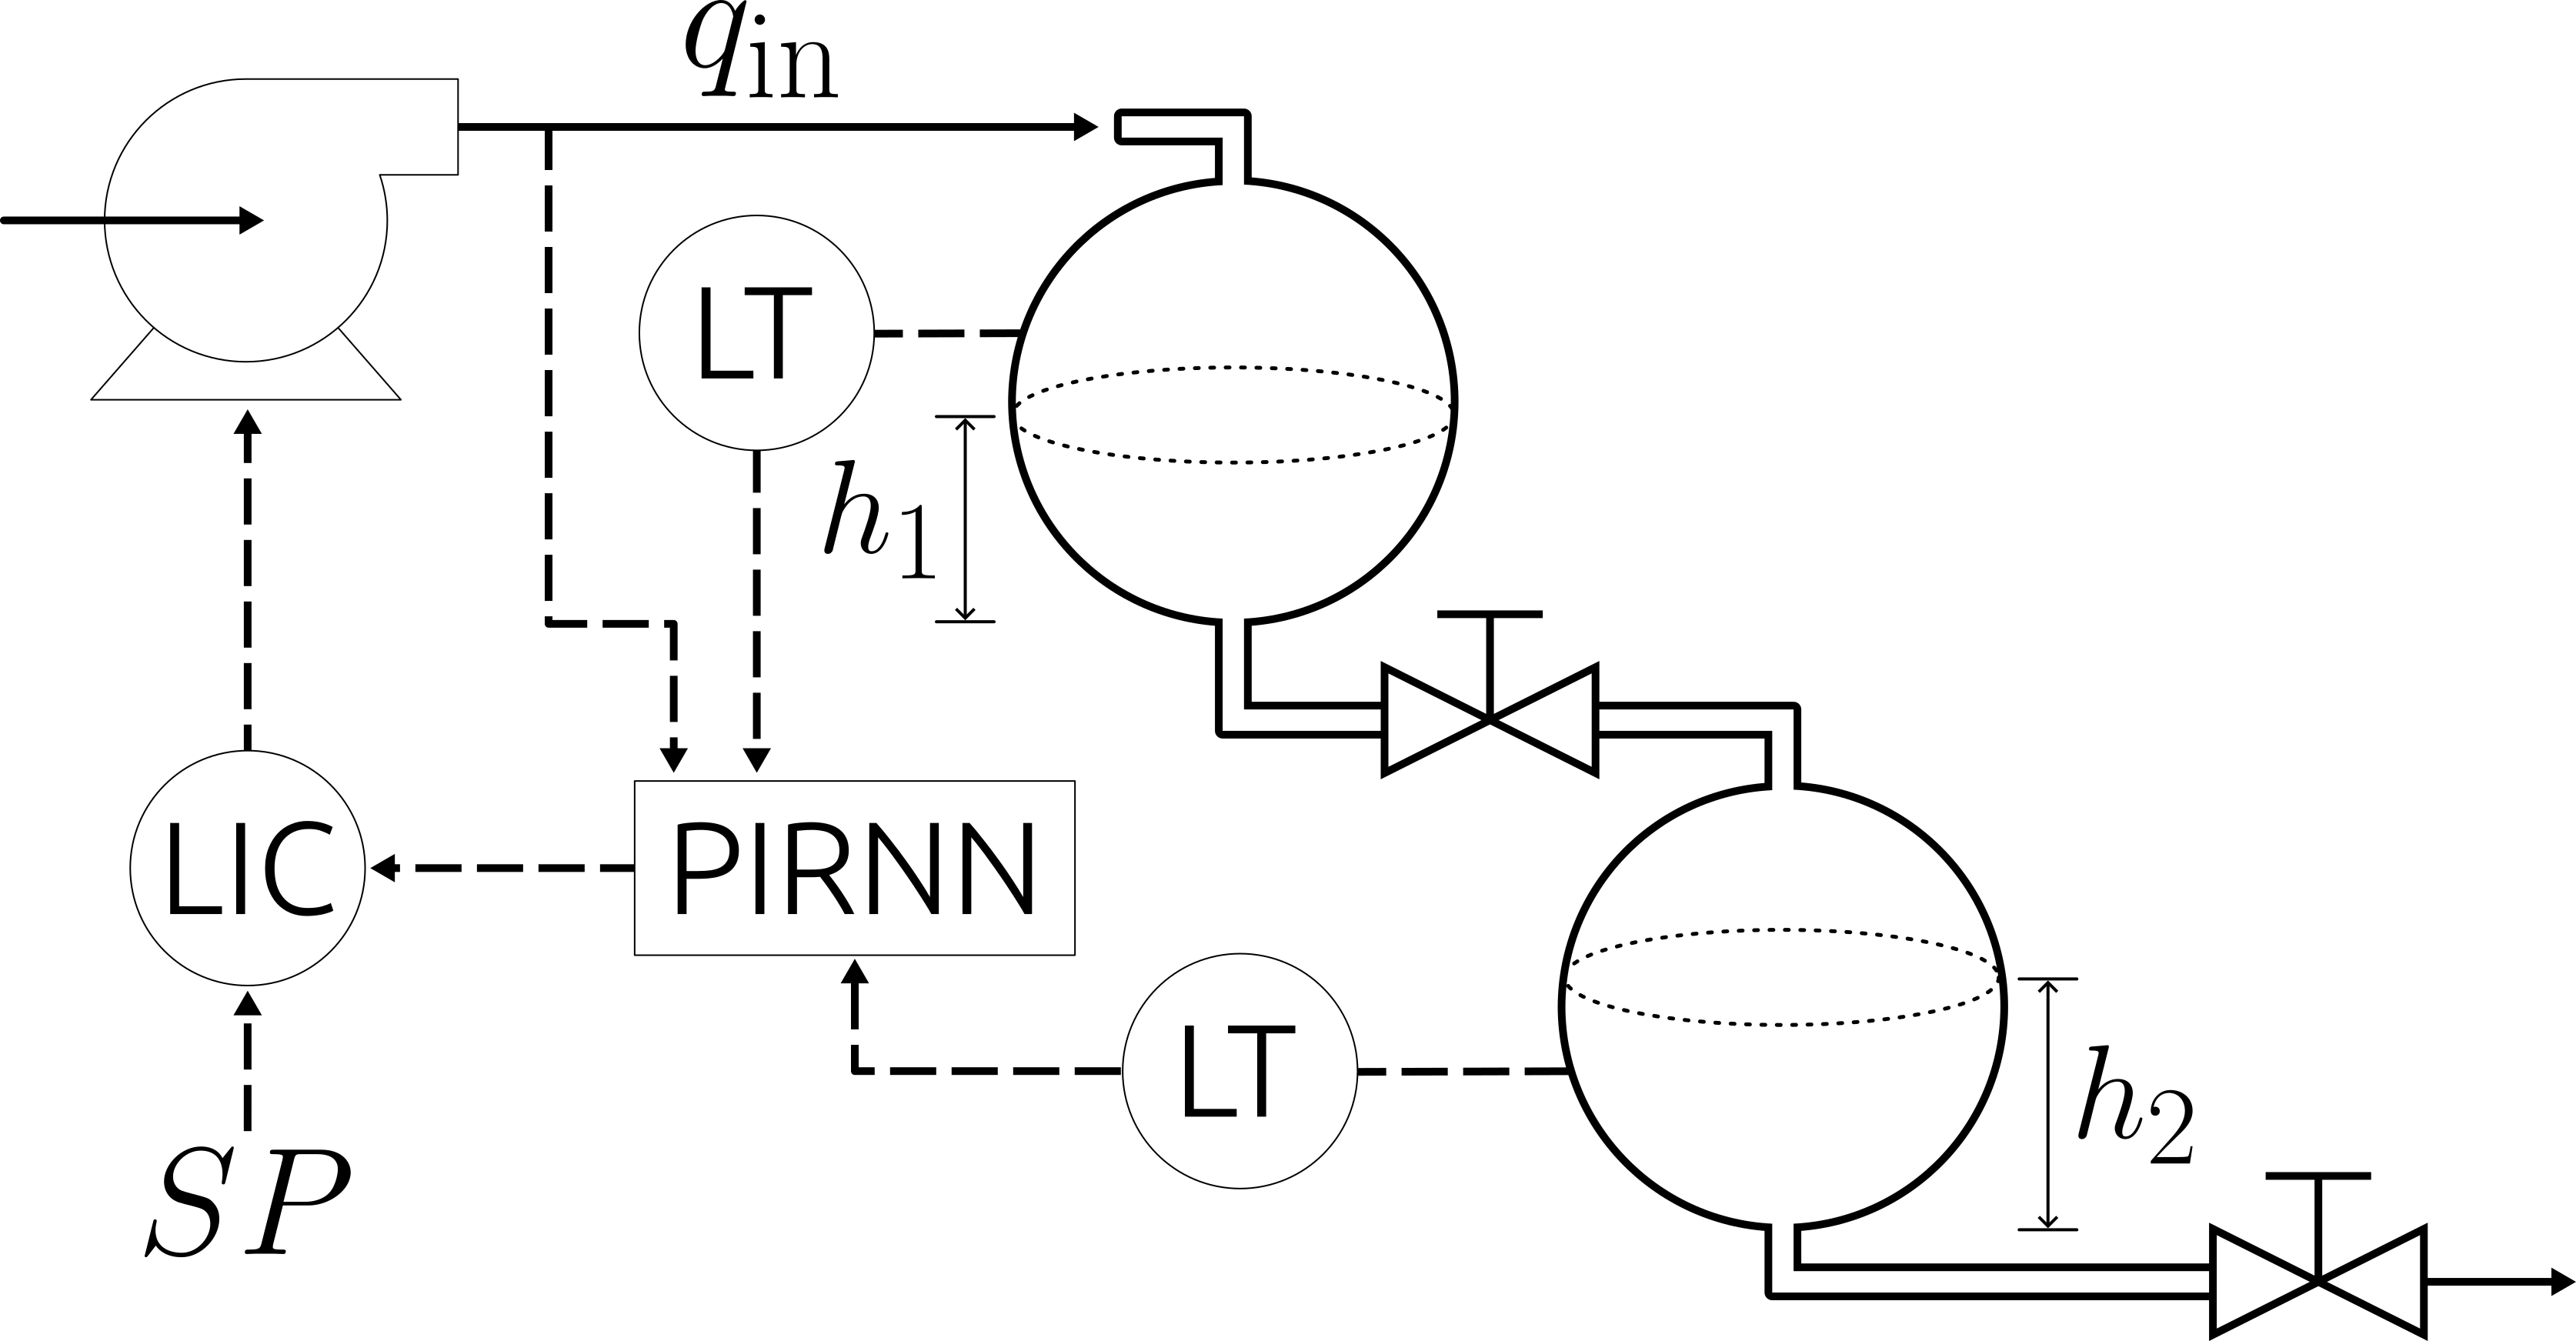
\includegraphics[width=0.45\textwidth]{process-diagram/full.png}
  \caption{Representação esquemática do sistema de dois tanques esféricos.}
  \label{fig:tank-system}
\end{figure}

A modelagem matemática dos tanques baseia-se no princípio de conservação de massa, do qual se obtêm \eqref{eq:tank_system_a} e \eqref{eq:tank_system_b}, que descrevem a variação temporal do nível de líquido em cada tanque.

\begin{subequations}
  \begin{align}
    \diff{h_1(t)}{t} & =
    \frac{
      q_{\mathrm{in}} - \alpha_1 s_1 \sqrt{2gh_1}
    }{
      \pi (2 R h_1 - h_1^2)
    }
    \label{eq:tank_system_a} \\[10pt]
    \diff{h_2(t)}{t} & =
    \frac{
      \alpha_1 s_1 \sqrt{2gh_1} - \alpha_2 s_2 \sqrt{2gh_2}
    }{
      \pi (2 R h_2 - h_2^2)
    }
    \label{eq:tank_system_b}
  \end{align}
\end{subequations}
%

O valor e a definição de cada constante utilizada na modelagem estão descritos na Tabela \ref{tab:tanks_params}.

\begin{table}[ht]
  \centering
  \caption{Constantes do sistema de equações diferenciais formado por \eqref{eq:tank_system_a} e \eqref{eq:tank_system_b}.}
  \label{tab:tanks_params}
  \begin{tabular}{ccc}
    \hline
    Símbolo    & Descrição                          & Valor            \\ \hline
    $\alpha_1$ & Coeficiente de fluxo da válvula 1  & 0,56             \\
    $\alpha_2$ & Coeficiente de fluxo da válvula 2  & 0,30             \\
    $s_1$      & Área da seção de saída do tanque 1 & 0,50 cm$^2$      \\
    $s_2$      & Área da seção de saída do tanque 2 & 0,50 cm$^2$      \\
    $g$        & Aceleração da gravidade            & 980,665 cm/s$^2$ \\
    $R$        & Raio dos tanques                   & 14,85 cm         \\ \hline
  \end{tabular}
\end{table}

\subsection{Estrutura da Rede Neural Artificial}

As Redes Neurais Recorrentes (\textit{Recurrent Neural Networks} — RNNs) são modelos computacionais projetados para processar dados sequenciais, sendo amplamente utilizadas em aplicações que envolvem séries temporais, reconhecimento de padrões e modelagem dinâmica de sistemas. Diferentemente das ANNs tradicionais, que tratam cada entrada de forma independente, as RNNs possuem conexões recorrentes que permitem reter informações de estados anteriores, possibilitando a captura de dependências temporais nos dados \citep{mienye_2024}.

No entanto, as RNNs compartilham algumas das limitações das redes neurais tradicionais. Seu desempenho depende fortemente da disponibilidade de um grande volume de dados representativos, o que nem sempre é viável. Outro ponto crítico é que esses modelos podem gerar previsões inconsistentes com o conhecimento científico disponível, pois não consideram explicitamente as leis físicas que regem o sistema \citep{karniadakis_2021}.

Para superar essas limitações surgiram as PIRNNs. Uma variação das PINNs que combina a capacidade das PINNs de incorporar conhecimento físico com a habilidade das RNNs de processar dados sequenciais e capturar dependências temporais eficientemente \citep{zheng_2023}. Elas funcionam de maneira semelhante às RNNs tradicionais, mas com a diferença de que, além do custo associado aos dados, a função de treinamento também considera o erro relativo ao problema físico. Dessa forma, a rede neural é penalizada sempre que suas previsões divergem das relações físicas conhecidas.

A PIRNN utilizada neste trabalho atua como um modelo dos dois tanques apresentados na Figura \ref{fig:tank-system}. A rede recebe como entrada os dois valores anteriores de três variáveis: os estados do sistema ($h_1$, $h_2$) e a vazão de entrada $q_{\mathrm{in}}$. Sua arquitetura, ilustrada na Figura \ref{fig:pirnn-diagram}, é composta por uma camada recorrente do tipo \textit{Elman} \citep{elman_1990} seguida por duas camadas totalmente conectadas, todas utilizando a função de ativação tangente hiperbólica ($\sigma$) e com 32 neurônios cada. Por fim, uma camada linear projeta o resultado para duas saídas, correspondentes aos próximos valores dos níveis dos tanques.

\begin{figure}[ht]
  \centering
  \resizebox{0.45\textwidth}{!}{% Graphic for TeX using PGF
% Title: /home/silas/Downloads/prh-35.1/LaTeX/common/figures/pirnn-diagram.dia
% Creator: Dia v0.97+git
% CreationDate: Tue May 20 14:37:33 2025
% For: silas
% \usepackage{tikz}
% The following commands are not supported in PSTricks at present
% We define them conditionally, so when they are implemented,
% this pgf file will use them.
\ifx\du\undefined
  \newlength{\du}
\fi
\setlength{\du}{15\unitlength}
\begin{tikzpicture}[even odd rule]
  \pgftransformxscale{1.000000}
  \pgftransformyscale{-1.000000}
  \definecolor{dialinecolor}{rgb}{0.000000, 0.000000, 0.000000}
  \pgfsetstrokecolor{dialinecolor}
  \pgfsetstrokeopacity{1.000000}
  \definecolor{diafillcolor}{rgb}{1.000000, 1.000000, 1.000000}
  \pgfsetfillcolor{diafillcolor}
  \pgfsetfillopacity{1.000000}
  \pgfsetlinewidth{0.100000\du}
  \pgfsetdash{}{0pt}
  \pgfsetmiterjoin
  \definecolor{diafillcolor}{rgb}{1.000000, 1.000000, 1.000000}
  \pgfsetfillcolor{diafillcolor}
  \pgfsetfillopacity{1.000000}
  \pgfpathellipse{\pgfpoint{29.000000\du}{16.000000\du}}{\pgfpoint{1.000000\du}{0\du}}{\pgfpoint{0\du}{1.000000\du}}
  \pgfusepath{fill}
  \definecolor{dialinecolor}{rgb}{0.000000, 0.000000, 0.000000}
  \pgfsetstrokecolor{dialinecolor}
  \pgfsetstrokeopacity{1.000000}
  \pgfpathellipse{\pgfpoint{29.000000\du}{16.000000\du}}{\pgfpoint{1.000000\du}{0\du}}{\pgfpoint{0\du}{1.000000\du}}
  \pgfusepath{stroke}
  % setfont left to latex
  \definecolor{dialinecolor}{rgb}{0.000000, 0.000000, 0.000000}
  \pgfsetstrokecolor{dialinecolor}
  \pgfsetstrokeopacity{1.000000}
  \definecolor{diafillcolor}{rgb}{0.000000, 0.000000, 0.000000}
  \pgfsetfillcolor{diafillcolor}
  \pgfsetfillopacity{1.000000}
  \node[anchor=base,inner sep=0pt, outer sep=0pt,color=dialinecolor] at (29.000000\du,16.194063\du){};
  \pgfsetlinewidth{0.100000\du}
  \pgfsetdash{}{0pt}
  \pgfsetmiterjoin
  \definecolor{diafillcolor}{rgb}{1.000000, 1.000000, 1.000000}
  \pgfsetfillcolor{diafillcolor}
  \pgfsetfillopacity{1.000000}
  \pgfpathellipse{\pgfpoint{33.000000\du}{18.000000\du}}{\pgfpoint{1.000000\du}{0\du}}{\pgfpoint{0\du}{1.000000\du}}
  \pgfusepath{fill}
  \definecolor{dialinecolor}{rgb}{0.000000, 0.000000, 0.000000}
  \pgfsetstrokecolor{dialinecolor}
  \pgfsetstrokeopacity{1.000000}
  \pgfpathellipse{\pgfpoint{33.000000\du}{18.000000\du}}{\pgfpoint{1.000000\du}{0\du}}{\pgfpoint{0\du}{1.000000\du}}
  \pgfusepath{stroke}
  % setfont left to latex
  \definecolor{dialinecolor}{rgb}{0.000000, 0.000000, 0.000000}
  \pgfsetstrokecolor{dialinecolor}
  \pgfsetstrokeopacity{1.000000}
  \definecolor{diafillcolor}{rgb}{0.000000, 0.000000, 0.000000}
  \pgfsetfillcolor{diafillcolor}
  \pgfsetfillopacity{1.000000}
  \node[anchor=base,inner sep=0pt, outer sep=0pt,color=dialinecolor] at (33.000000\du,18.194063\du){};
  \pgfsetlinewidth{0.100000\du}
  \pgfsetdash{}{0pt}
  \pgfsetmiterjoin
  \definecolor{diafillcolor}{rgb}{1.000000, 1.000000, 1.000000}
  \pgfsetfillcolor{diafillcolor}
  \pgfsetfillopacity{1.000000}
  \pgfpathellipse{\pgfpoint{33.000000\du}{23.000000\du}}{\pgfpoint{1.000000\du}{0\du}}{\pgfpoint{0\du}{1.000000\du}}
  \pgfusepath{fill}
  \definecolor{dialinecolor}{rgb}{0.000000, 0.000000, 0.000000}
  \pgfsetstrokecolor{dialinecolor}
  \pgfsetstrokeopacity{1.000000}
  \pgfpathellipse{\pgfpoint{33.000000\du}{23.000000\du}}{\pgfpoint{1.000000\du}{0\du}}{\pgfpoint{0\du}{1.000000\du}}
  \pgfusepath{stroke}
  % setfont left to latex
  \definecolor{dialinecolor}{rgb}{0.000000, 0.000000, 0.000000}
  \pgfsetstrokecolor{dialinecolor}
  \pgfsetstrokeopacity{1.000000}
  \definecolor{diafillcolor}{rgb}{0.000000, 0.000000, 0.000000}
  \pgfsetfillcolor{diafillcolor}
  \pgfsetfillopacity{1.000000}
  \node[anchor=base,inner sep=0pt, outer sep=0pt,color=dialinecolor] at (33.000000\du,23.194063\du){};
  % setfont left to latex
  \definecolor{dialinecolor}{rgb}{0.000000, 0.000000, 0.000000}
  \pgfsetstrokecolor{dialinecolor}
  \pgfsetstrokeopacity{1.000000}
  \definecolor{diafillcolor}{rgb}{0.000000, 0.000000, 0.000000}
  \pgfsetfillcolor{diafillcolor}
  \pgfsetfillopacity{1.000000}
  \node[anchor=base,inner sep=0pt, outer sep=0pt,color=dialinecolor] at (33.000000\du,18.221562\du){$h_1^{(t)}$};
  % setfont left to latex
  \definecolor{dialinecolor}{rgb}{0.000000, 0.000000, 0.000000}
  \pgfsetstrokecolor{dialinecolor}
  \pgfsetstrokeopacity{1.000000}
  \definecolor{diafillcolor}{rgb}{0.000000, 0.000000, 0.000000}
  \pgfsetfillcolor{diafillcolor}
  \pgfsetfillopacity{1.000000}
  \node[anchor=base,inner sep=0pt, outer sep=0pt,color=dialinecolor] at (33.000000\du,23.221562\du){$h_2^{(t)}$};
  % setfont left to latex
  \definecolor{dialinecolor}{rgb}{0.000000, 0.000000, 0.000000}
  \pgfsetstrokecolor{dialinecolor}
  \pgfsetstrokeopacity{1.000000}
  \definecolor{diafillcolor}{rgb}{0.000000, 0.000000, 0.000000}
  \pgfsetfillcolor{diafillcolor}
  \pgfsetfillopacity{1.000000}
  \node[anchor=base west,inner sep=0pt,outer sep=0pt,color=dialinecolor] at (33.000000\du,18.000000\du){};
  \pgfsetlinewidth{0.100000\du}
  \pgfsetdash{}{0pt}
  \pgfsetmiterjoin
  {\pgfsetcornersarced{\pgfpoint{1.000000\du}{1.000000\du}}\definecolor{diafillcolor}{rgb}{1.000000, 1.000000, 1.000000}
    \pgfsetfillcolor{diafillcolor}
    \pgfsetfillopacity{1.000000}
    \fill (12.500000\du,15.500000\du)--(12.500000\du,17.500000\du)--(17.500000\du,17.500000\du)--(17.500000\du,15.500000\du)--cycle;
  }{\pgfsetcornersarced{\pgfpoint{1.000000\du}{1.000000\du}}\definecolor{dialinecolor}{rgb}{0.000000, 0.000000, 0.000000}
    \pgfsetstrokecolor{dialinecolor}
    \pgfsetstrokeopacity{1.000000}
    \draw (12.500000\du,15.500000\du)--(12.500000\du,17.500000\du)--(17.500000\du,17.500000\du)--(17.500000\du,15.500000\du)--cycle;
  }% setfont left to latex
  \definecolor{dialinecolor}{rgb}{0.000000, 0.000000, 0.000000}
  \pgfsetstrokecolor{dialinecolor}
  \pgfsetstrokeopacity{1.000000}
  \definecolor{diafillcolor}{rgb}{0.000000, 0.000000, 0.000000}
  \pgfsetfillcolor{diafillcolor}
  \pgfsetfillopacity{1.000000}
  \node[anchor=base,inner sep=0pt, outer sep=0pt,color=dialinecolor] at (15.000000\du,16.694063\du){};
  % setfont left to latex
  \definecolor{dialinecolor}{rgb}{0.000000, 0.000000, 0.000000}
  \pgfsetstrokecolor{dialinecolor}
  \pgfsetstrokeopacity{1.000000}
  \definecolor{diafillcolor}{rgb}{0.000000, 0.000000, 0.000000}
  \pgfsetfillcolor{diafillcolor}
  \pgfsetfillopacity{1.000000}
  \node[anchor=base,inner sep=0pt, outer sep=0pt,color=dialinecolor] at (15.000000\du,16.721562\du){$[h_1^{(t-2)}, h_1^{(t-1)}]$};
  \pgfsetlinewidth{0.100000\du}
  \pgfsetdash{}{0pt}
  \pgfsetmiterjoin
  {\pgfsetcornersarced{\pgfpoint{1.000000\du}{1.000000\du}}\definecolor{diafillcolor}{rgb}{1.000000, 1.000000, 1.000000}
    \pgfsetfillcolor{diafillcolor}
    \pgfsetfillopacity{1.000000}
    \fill (12.500000\du,19.500000\du)--(12.500000\du,21.500000\du)--(17.500000\du,21.500000\du)--(17.500000\du,19.500000\du)--cycle;
  }{\pgfsetcornersarced{\pgfpoint{1.000000\du}{1.000000\du}}\definecolor{dialinecolor}{rgb}{0.000000, 0.000000, 0.000000}
    \pgfsetstrokecolor{dialinecolor}
    \pgfsetstrokeopacity{1.000000}
    \draw (12.500000\du,19.500000\du)--(12.500000\du,21.500000\du)--(17.500000\du,21.500000\du)--(17.500000\du,19.500000\du)--cycle;
  }% setfont left to latex
  \definecolor{dialinecolor}{rgb}{0.000000, 0.000000, 0.000000}
  \pgfsetstrokecolor{dialinecolor}
  \pgfsetstrokeopacity{1.000000}
  \definecolor{diafillcolor}{rgb}{0.000000, 0.000000, 0.000000}
  \pgfsetfillcolor{diafillcolor}
  \pgfsetfillopacity{1.000000}
  \node[anchor=base,inner sep=0pt, outer sep=0pt,color=dialinecolor] at (15.000000\du,20.694063\du){};
  \pgfsetlinewidth{0.100000\du}
  \pgfsetdash{}{0pt}
  \pgfsetmiterjoin
  {\pgfsetcornersarced{\pgfpoint{1.000000\du}{1.000000\du}}\definecolor{diafillcolor}{rgb}{1.000000, 1.000000, 1.000000}
    \pgfsetfillcolor{diafillcolor}
    \pgfsetfillopacity{1.000000}
    \fill (12.500000\du,23.500000\du)--(12.500000\du,25.500000\du)--(17.500000\du,25.500000\du)--(17.500000\du,23.500000\du)--cycle;
  }{\pgfsetcornersarced{\pgfpoint{1.000000\du}{1.000000\du}}\definecolor{dialinecolor}{rgb}{0.000000, 0.000000, 0.000000}
    \pgfsetstrokecolor{dialinecolor}
    \pgfsetstrokeopacity{1.000000}
    \draw (12.500000\du,23.500000\du)--(12.500000\du,25.500000\du)--(17.500000\du,25.500000\du)--(17.500000\du,23.500000\du)--cycle;
  }% setfont left to latex
  \definecolor{dialinecolor}{rgb}{0.000000, 0.000000, 0.000000}
  \pgfsetstrokecolor{dialinecolor}
  \pgfsetstrokeopacity{1.000000}
  \definecolor{diafillcolor}{rgb}{0.000000, 0.000000, 0.000000}
  \pgfsetfillcolor{diafillcolor}
  \pgfsetfillopacity{1.000000}
  \node[anchor=base,inner sep=0pt, outer sep=0pt,color=dialinecolor] at (15.000000\du,24.694063\du){};
  % setfont left to latex
  \definecolor{dialinecolor}{rgb}{0.000000, 0.000000, 0.000000}
  \pgfsetstrokecolor{dialinecolor}
  \pgfsetstrokeopacity{1.000000}
  \definecolor{diafillcolor}{rgb}{0.000000, 0.000000, 0.000000}
  \pgfsetfillcolor{diafillcolor}
  \pgfsetfillopacity{1.000000}
  \node[anchor=base,inner sep=0pt, outer sep=0pt,color=dialinecolor] at (15.000000\du,20.721562\du){$[h_2^{(t-2)}, h_2^{(t-1)}]$};
  % setfont left to latex
  \definecolor{dialinecolor}{rgb}{0.000000, 0.000000, 0.000000}
  \pgfsetstrokecolor{dialinecolor}
  \pgfsetstrokeopacity{1.000000}
  \definecolor{diafillcolor}{rgb}{0.000000, 0.000000, 0.000000}
  \pgfsetfillcolor{diafillcolor}
  \pgfsetfillopacity{1.000000}
  \node[anchor=base,inner sep=0pt, outer sep=0pt,color=dialinecolor] at (15.000000\du,24.721562\du){$[q_{\mathrm{in}}^{(t-2)}, q_{\mathrm{in}}^{(t-1)}]$};
  % setfont left to latex
  \definecolor{dialinecolor}{rgb}{0.000000, 0.000000, 0.000000}
  \pgfsetstrokecolor{dialinecolor}
  \pgfsetstrokeopacity{1.000000}
  \definecolor{diafillcolor}{rgb}{0.000000, 0.000000, 0.000000}
  \pgfsetfillcolor{diafillcolor}
  \pgfsetfillopacity{1.000000}
  \node[anchor=base,inner sep=0pt, outer sep=0pt,color=dialinecolor] at (21.000000\du,27.221562\du){Camada RNN};
  \pgfsetlinewidth{0.100000\du}
  \pgfsetdash{}{0pt}
  \pgfsetmiterjoin
  \definecolor{diafillcolor}{rgb}{1.000000, 1.000000, 1.000000}
  \pgfsetfillcolor{diafillcolor}
  \pgfsetfillopacity{1.000000}
  \pgfpathellipse{\pgfpoint{25.000000\du}{16.000000\du}}{\pgfpoint{1.000000\du}{0\du}}{\pgfpoint{0\du}{1.000000\du}}
  \pgfusepath{fill}
  \definecolor{dialinecolor}{rgb}{0.000000, 0.000000, 0.000000}
  \pgfsetstrokecolor{dialinecolor}
  \pgfsetstrokeopacity{1.000000}
  \pgfpathellipse{\pgfpoint{25.000000\du}{16.000000\du}}{\pgfpoint{1.000000\du}{0\du}}{\pgfpoint{0\du}{1.000000\du}}
  \pgfusepath{stroke}
  % setfont left to latex
  \definecolor{dialinecolor}{rgb}{0.000000, 0.000000, 0.000000}
  \pgfsetstrokecolor{dialinecolor}
  \pgfsetstrokeopacity{1.000000}
  \definecolor{diafillcolor}{rgb}{0.000000, 0.000000, 0.000000}
  \pgfsetfillcolor{diafillcolor}
  \pgfsetfillopacity{1.000000}
  \node[anchor=base,inner sep=0pt, outer sep=0pt,color=dialinecolor] at (25.000000\du,16.194063\du){};
  \pgfsetlinewidth{0.100000\du}
  \pgfsetdash{}{0pt}
  \pgfsetmiterjoin
  \definecolor{diafillcolor}{rgb}{1.000000, 1.000000, 1.000000}
  \pgfsetfillcolor{diafillcolor}
  \pgfsetfillopacity{1.000000}
  \pgfpathellipse{\pgfpoint{25.000000\du}{19.000000\du}}{\pgfpoint{1.000000\du}{0\du}}{\pgfpoint{0\du}{1.000000\du}}
  \pgfusepath{fill}
  \definecolor{dialinecolor}{rgb}{0.000000, 0.000000, 0.000000}
  \pgfsetstrokecolor{dialinecolor}
  \pgfsetstrokeopacity{1.000000}
  \pgfpathellipse{\pgfpoint{25.000000\du}{19.000000\du}}{\pgfpoint{1.000000\du}{0\du}}{\pgfpoint{0\du}{1.000000\du}}
  \pgfusepath{stroke}
  % setfont left to latex
  \definecolor{dialinecolor}{rgb}{0.000000, 0.000000, 0.000000}
  \pgfsetstrokecolor{dialinecolor}
  \pgfsetstrokeopacity{1.000000}
  \definecolor{diafillcolor}{rgb}{0.000000, 0.000000, 0.000000}
  \pgfsetfillcolor{diafillcolor}
  \pgfsetfillopacity{1.000000}
  \node[anchor=base,inner sep=0pt, outer sep=0pt,color=dialinecolor] at (25.000000\du,19.194063\du){};
  \pgfsetlinewidth{0.100000\du}
  \pgfsetdash{}{0pt}
  \pgfsetmiterjoin
  \definecolor{diafillcolor}{rgb}{1.000000, 1.000000, 1.000000}
  \pgfsetfillcolor{diafillcolor}
  \pgfsetfillopacity{1.000000}
  \pgfpathellipse{\pgfpoint{25.000000\du}{25.000000\du}}{\pgfpoint{1.000000\du}{0\du}}{\pgfpoint{0\du}{1.000000\du}}
  \pgfusepath{fill}
  \definecolor{dialinecolor}{rgb}{0.000000, 0.000000, 0.000000}
  \pgfsetstrokecolor{dialinecolor}
  \pgfsetstrokeopacity{1.000000}
  \pgfpathellipse{\pgfpoint{25.000000\du}{25.000000\du}}{\pgfpoint{1.000000\du}{0\du}}{\pgfpoint{0\du}{1.000000\du}}
  \pgfusepath{stroke}
  % setfont left to latex
  \definecolor{dialinecolor}{rgb}{0.000000, 0.000000, 0.000000}
  \pgfsetstrokecolor{dialinecolor}
  \pgfsetstrokeopacity{1.000000}
  \definecolor{diafillcolor}{rgb}{0.000000, 0.000000, 0.000000}
  \pgfsetfillcolor{diafillcolor}
  \pgfsetfillopacity{1.000000}
  \node[anchor=base,inner sep=0pt, outer sep=0pt,color=dialinecolor] at (25.000000\du,25.194063\du){};
  \pgfsetlinewidth{0.100000\du}
  \pgfsetdash{}{0pt}
  \pgfsetbuttcap
  {
    \definecolor{diafillcolor}{rgb}{0.000000, 0.000000, 0.000000}
    \pgfsetfillcolor{diafillcolor}
    \pgfsetfillopacity{1.000000}
    % was here!!!
    \pgfsetarrowsend{stealth}
    \definecolor{dialinecolor}{rgb}{0.000000, 0.000000, 0.000000}
    \pgfsetstrokecolor{dialinecolor}
    \pgfsetstrokeopacity{1.000000}
    \draw (22.000000\du,19.000000\du)--(24.000000\du,19.000000\du);
  }
  % setfont left to latex
  \definecolor{dialinecolor}{rgb}{0.000000, 0.000000, 0.000000}
  \pgfsetstrokecolor{dialinecolor}
  \pgfsetstrokeopacity{1.000000}
  \definecolor{diafillcolor}{rgb}{0.000000, 0.000000, 0.000000}
  \pgfsetfillcolor{diafillcolor}
  \pgfsetfillopacity{1.000000}
  \node[anchor=base,inner sep=0pt, outer sep=0pt,color=dialinecolor] at (25.000000\du,21.421563\du){.};
  % setfont left to latex
  \definecolor{dialinecolor}{rgb}{0.000000, 0.000000, 0.000000}
  \pgfsetstrokecolor{dialinecolor}
  \pgfsetstrokeopacity{1.000000}
  \definecolor{diafillcolor}{rgb}{0.000000, 0.000000, 0.000000}
  \pgfsetfillcolor{diafillcolor}
  \pgfsetfillopacity{1.000000}
  \node[anchor=base,inner sep=0pt, outer sep=0pt,color=dialinecolor] at (25.000000\du,22.221563\du){.};
  % setfont left to latex
  \definecolor{dialinecolor}{rgb}{0.000000, 0.000000, 0.000000}
  \pgfsetstrokecolor{dialinecolor}
  \pgfsetstrokeopacity{1.000000}
  \definecolor{diafillcolor}{rgb}{0.000000, 0.000000, 0.000000}
  \pgfsetfillcolor{diafillcolor}
  \pgfsetfillopacity{1.000000}
  \node[anchor=base,inner sep=0pt, outer sep=0pt,color=dialinecolor] at (25.000000\du,23.021563\du){.};
  % setfont left to latex
  \definecolor{dialinecolor}{rgb}{0.000000, 0.000000, 0.000000}
  \pgfsetstrokecolor{dialinecolor}
  \pgfsetstrokeopacity{1.000000}
  \definecolor{diafillcolor}{rgb}{0.000000, 0.000000, 0.000000}
  \pgfsetfillcolor{diafillcolor}
  \pgfsetfillopacity{1.000000}
  \node[anchor=base,inner sep=0pt, outer sep=0pt,color=dialinecolor] at (25.000000\du,16.221562\du){$\sigma$};
  % setfont left to latex
  \definecolor{dialinecolor}{rgb}{0.000000, 0.000000, 0.000000}
  \pgfsetstrokecolor{dialinecolor}
  \pgfsetstrokeopacity{1.000000}
  \definecolor{diafillcolor}{rgb}{0.000000, 0.000000, 0.000000}
  \pgfsetfillcolor{diafillcolor}
  \pgfsetfillopacity{1.000000}
  \node[anchor=base,inner sep=0pt, outer sep=0pt,color=dialinecolor] at (25.000000\du,19.221562\du){$\sigma$};
  % setfont left to latex
  \definecolor{dialinecolor}{rgb}{0.000000, 0.000000, 0.000000}
  \pgfsetstrokecolor{dialinecolor}
  \pgfsetstrokeopacity{1.000000}
  \definecolor{diafillcolor}{rgb}{0.000000, 0.000000, 0.000000}
  \pgfsetfillcolor{diafillcolor}
  \pgfsetfillopacity{1.000000}
  \node[anchor=base,inner sep=0pt, outer sep=0pt,color=dialinecolor] at (25.000000\du,25.221562\du){$\sigma$};
  \pgfsetlinewidth{0.100000\du}
  \pgfsetdash{}{0pt}
  \pgfsetmiterjoin
  \definecolor{diafillcolor}{rgb}{1.000000, 1.000000, 1.000000}
  \pgfsetfillcolor{diafillcolor}
  \pgfsetfillopacity{1.000000}
  \pgfpathellipse{\pgfpoint{21.000000\du}{16.000000\du}}{\pgfpoint{1.000000\du}{0\du}}{\pgfpoint{0\du}{1.000000\du}}
  \pgfusepath{fill}
  \definecolor{dialinecolor}{rgb}{0.000000, 0.000000, 0.000000}
  \pgfsetstrokecolor{dialinecolor}
  \pgfsetstrokeopacity{1.000000}
  \pgfpathellipse{\pgfpoint{21.000000\du}{16.000000\du}}{\pgfpoint{1.000000\du}{0\du}}{\pgfpoint{0\du}{1.000000\du}}
  \pgfusepath{stroke}
  % setfont left to latex
  \definecolor{dialinecolor}{rgb}{0.000000, 0.000000, 0.000000}
  \pgfsetstrokecolor{dialinecolor}
  \pgfsetstrokeopacity{1.000000}
  \definecolor{diafillcolor}{rgb}{0.000000, 0.000000, 0.000000}
  \pgfsetfillcolor{diafillcolor}
  \pgfsetfillopacity{1.000000}
  \node[anchor=base,inner sep=0pt, outer sep=0pt,color=dialinecolor] at (21.000000\du,16.194063\du){};
  \pgfsetlinewidth{0.100000\du}
  \pgfsetdash{}{0pt}
  \pgfsetmiterjoin
  \definecolor{diafillcolor}{rgb}{1.000000, 1.000000, 1.000000}
  \pgfsetfillcolor{diafillcolor}
  \pgfsetfillopacity{1.000000}
  \pgfpathellipse{\pgfpoint{21.000000\du}{19.000000\du}}{\pgfpoint{1.000000\du}{0\du}}{\pgfpoint{0\du}{1.000000\du}}
  \pgfusepath{fill}
  \definecolor{dialinecolor}{rgb}{0.000000, 0.000000, 0.000000}
  \pgfsetstrokecolor{dialinecolor}
  \pgfsetstrokeopacity{1.000000}
  \pgfpathellipse{\pgfpoint{21.000000\du}{19.000000\du}}{\pgfpoint{1.000000\du}{0\du}}{\pgfpoint{0\du}{1.000000\du}}
  \pgfusepath{stroke}
  % setfont left to latex
  \definecolor{dialinecolor}{rgb}{0.000000, 0.000000, 0.000000}
  \pgfsetstrokecolor{dialinecolor}
  \pgfsetstrokeopacity{1.000000}
  \definecolor{diafillcolor}{rgb}{0.000000, 0.000000, 0.000000}
  \pgfsetfillcolor{diafillcolor}
  \pgfsetfillopacity{1.000000}
  \node[anchor=base,inner sep=0pt, outer sep=0pt,color=dialinecolor] at (21.000000\du,19.194063\du){};
  \pgfsetlinewidth{0.100000\du}
  \pgfsetdash{}{0pt}
  \pgfsetmiterjoin
  \definecolor{diafillcolor}{rgb}{1.000000, 1.000000, 1.000000}
  \pgfsetfillcolor{diafillcolor}
  \pgfsetfillopacity{1.000000}
  \pgfpathellipse{\pgfpoint{21.000000\du}{25.000000\du}}{\pgfpoint{1.000000\du}{0\du}}{\pgfpoint{0\du}{1.000000\du}}
  \pgfusepath{fill}
  \definecolor{dialinecolor}{rgb}{0.000000, 0.000000, 0.000000}
  \pgfsetstrokecolor{dialinecolor}
  \pgfsetstrokeopacity{1.000000}
  \pgfpathellipse{\pgfpoint{21.000000\du}{25.000000\du}}{\pgfpoint{1.000000\du}{0\du}}{\pgfpoint{0\du}{1.000000\du}}
  \pgfusepath{stroke}
  % setfont left to latex
  \definecolor{dialinecolor}{rgb}{0.000000, 0.000000, 0.000000}
  \pgfsetstrokecolor{dialinecolor}
  \pgfsetstrokeopacity{1.000000}
  \definecolor{diafillcolor}{rgb}{0.000000, 0.000000, 0.000000}
  \pgfsetfillcolor{diafillcolor}
  \pgfsetfillopacity{1.000000}
  \node[anchor=base,inner sep=0pt, outer sep=0pt,color=dialinecolor] at (21.000000\du,25.194063\du){};
  % setfont left to latex
  \definecolor{dialinecolor}{rgb}{0.000000, 0.000000, 0.000000}
  \pgfsetstrokecolor{dialinecolor}
  \pgfsetstrokeopacity{1.000000}
  \definecolor{diafillcolor}{rgb}{0.000000, 0.000000, 0.000000}
  \pgfsetfillcolor{diafillcolor}
  \pgfsetfillopacity{1.000000}
  \node[anchor=base,inner sep=0pt, outer sep=0pt,color=dialinecolor] at (21.000000\du,21.421563\du){.};
  % setfont left to latex
  \definecolor{dialinecolor}{rgb}{0.000000, 0.000000, 0.000000}
  \pgfsetstrokecolor{dialinecolor}
  \pgfsetstrokeopacity{1.000000}
  \definecolor{diafillcolor}{rgb}{0.000000, 0.000000, 0.000000}
  \pgfsetfillcolor{diafillcolor}
  \pgfsetfillopacity{1.000000}
  \node[anchor=base,inner sep=0pt, outer sep=0pt,color=dialinecolor] at (21.000000\du,22.221563\du){.};
  % setfont left to latex
  \definecolor{dialinecolor}{rgb}{0.000000, 0.000000, 0.000000}
  \pgfsetstrokecolor{dialinecolor}
  \pgfsetstrokeopacity{1.000000}
  \definecolor{diafillcolor}{rgb}{0.000000, 0.000000, 0.000000}
  \pgfsetfillcolor{diafillcolor}
  \pgfsetfillopacity{1.000000}
  \node[anchor=base,inner sep=0pt, outer sep=0pt,color=dialinecolor] at (21.000000\du,23.021563\du){.};
  % setfont left to latex
  \definecolor{dialinecolor}{rgb}{0.000000, 0.000000, 0.000000}
  \pgfsetstrokecolor{dialinecolor}
  \pgfsetstrokeopacity{1.000000}
  \definecolor{diafillcolor}{rgb}{0.000000, 0.000000, 0.000000}
  \pgfsetfillcolor{diafillcolor}
  \pgfsetfillopacity{1.000000}
  \node[anchor=base,inner sep=0pt, outer sep=0pt,color=dialinecolor] at (21.000000\du,16.221562\du){$\sigma$};
  % setfont left to latex
  \definecolor{dialinecolor}{rgb}{0.000000, 0.000000, 0.000000}
  \pgfsetstrokecolor{dialinecolor}
  \pgfsetstrokeopacity{1.000000}
  \definecolor{diafillcolor}{rgb}{0.000000, 0.000000, 0.000000}
  \pgfsetfillcolor{diafillcolor}
  \pgfsetfillopacity{1.000000}
  \node[anchor=base,inner sep=0pt, outer sep=0pt,color=dialinecolor] at (21.000000\du,19.221562\du){$\sigma$};
  % setfont left to latex
  \definecolor{dialinecolor}{rgb}{0.000000, 0.000000, 0.000000}
  \pgfsetstrokecolor{dialinecolor}
  \pgfsetstrokeopacity{1.000000}
  \definecolor{diafillcolor}{rgb}{0.000000, 0.000000, 0.000000}
  \pgfsetfillcolor{diafillcolor}
  \pgfsetfillopacity{1.000000}
  \node[anchor=base,inner sep=0pt, outer sep=0pt,color=dialinecolor] at (21.000000\du,25.221562\du){$\sigma$};
  \pgfsetlinewidth{0.100000\du}
  \pgfsetdash{}{0pt}
  \pgfsetmiterjoin
  \pgfsetbuttcap
  {
    \definecolor{diafillcolor}{rgb}{0.000000, 0.000000, 0.000000}
    \pgfsetfillcolor{diafillcolor}
    \pgfsetfillopacity{1.000000}
    % was here!!!
    \pgfsetarrowsend{stealth}
    \definecolor{dialinecolor}{rgb}{0.000000, 0.000000, 0.000000}
    \pgfsetstrokecolor{dialinecolor}
    \pgfsetstrokeopacity{1.000000}
    \pgfpathmoveto{\pgfpoint{21.000000\du}{15.000000\du}}
    \pgfpathcurveto{\pgfpoint{21.000000\du}{14.000000\du}}{\pgfpoint{22.207100\du}{13.792900\du}}{\pgfpoint{21.707100\du}{15.292900\du}}
    \pgfusepath{stroke}
  }
  \pgfsetlinewidth{0.100000\du}
  \pgfsetdash{}{0pt}
  \pgfsetmiterjoin
  \pgfsetbuttcap
  {
    \definecolor{diafillcolor}{rgb}{0.000000, 0.000000, 0.000000}
    \pgfsetfillcolor{diafillcolor}
    \pgfsetfillopacity{1.000000}
    % was here!!!
    \pgfsetarrowsend{stealth}
    \definecolor{dialinecolor}{rgb}{0.000000, 0.000000, 0.000000}
    \pgfsetstrokecolor{dialinecolor}
    \pgfsetstrokeopacity{1.000000}
    \pgfpathmoveto{\pgfpoint{21.000000\du}{18.000000\du}}
    \pgfpathcurveto{\pgfpoint{21.000000\du}{17.000000\du}}{\pgfpoint{22.207100\du}{16.792900\du}}{\pgfpoint{21.707100\du}{18.292900\du}}
    \pgfusepath{stroke}
  }
  \pgfsetlinewidth{0.100000\du}
  \pgfsetdash{}{0pt}
  \pgfsetmiterjoin
  \pgfsetbuttcap
  {
    \definecolor{diafillcolor}{rgb}{0.000000, 0.000000, 0.000000}
    \pgfsetfillcolor{diafillcolor}
    \pgfsetfillopacity{1.000000}
    % was here!!!
    \pgfsetarrowsend{stealth}
    \definecolor{dialinecolor}{rgb}{0.000000, 0.000000, 0.000000}
    \pgfsetstrokecolor{dialinecolor}
    \pgfsetstrokeopacity{1.000000}
    \pgfpathmoveto{\pgfpoint{21.000000\du}{24.000000\du}}
    \pgfpathcurveto{\pgfpoint{21.000000\du}{23.000000\du}}{\pgfpoint{22.207100\du}{22.792900\du}}{\pgfpoint{21.707100\du}{24.292900\du}}
    \pgfusepath{stroke}
  }
  \pgfsetlinewidth{0.100000\du}
  \pgfsetdash{}{0pt}
  \pgfsetmiterjoin
  \definecolor{diafillcolor}{rgb}{1.000000, 1.000000, 1.000000}
  \pgfsetfillcolor{diafillcolor}
  \pgfsetfillopacity{1.000000}
  \pgfpathellipse{\pgfpoint{29.000000\du}{19.000000\du}}{\pgfpoint{1.000000\du}{0\du}}{\pgfpoint{0\du}{1.000000\du}}
  \pgfusepath{fill}
  \definecolor{dialinecolor}{rgb}{0.000000, 0.000000, 0.000000}
  \pgfsetstrokecolor{dialinecolor}
  \pgfsetstrokeopacity{1.000000}
  \pgfpathellipse{\pgfpoint{29.000000\du}{19.000000\du}}{\pgfpoint{1.000000\du}{0\du}}{\pgfpoint{0\du}{1.000000\du}}
  \pgfusepath{stroke}
  % setfont left to latex
  \definecolor{dialinecolor}{rgb}{0.000000, 0.000000, 0.000000}
  \pgfsetstrokecolor{dialinecolor}
  \pgfsetstrokeopacity{1.000000}
  \definecolor{diafillcolor}{rgb}{0.000000, 0.000000, 0.000000}
  \pgfsetfillcolor{diafillcolor}
  \pgfsetfillopacity{1.000000}
  \node[anchor=base,inner sep=0pt, outer sep=0pt,color=dialinecolor] at (29.000000\du,19.194063\du){};
  \pgfsetlinewidth{0.100000\du}
  \pgfsetdash{}{0pt}
  \pgfsetmiterjoin
  \definecolor{diafillcolor}{rgb}{1.000000, 1.000000, 1.000000}
  \pgfsetfillcolor{diafillcolor}
  \pgfsetfillopacity{1.000000}
  \pgfpathellipse{\pgfpoint{29.000000\du}{25.000000\du}}{\pgfpoint{1.000000\du}{0\du}}{\pgfpoint{0\du}{1.000000\du}}
  \pgfusepath{fill}
  \definecolor{dialinecolor}{rgb}{0.000000, 0.000000, 0.000000}
  \pgfsetstrokecolor{dialinecolor}
  \pgfsetstrokeopacity{1.000000}
  \pgfpathellipse{\pgfpoint{29.000000\du}{25.000000\du}}{\pgfpoint{1.000000\du}{0\du}}{\pgfpoint{0\du}{1.000000\du}}
  \pgfusepath{stroke}
  % setfont left to latex
  \definecolor{dialinecolor}{rgb}{0.000000, 0.000000, 0.000000}
  \pgfsetstrokecolor{dialinecolor}
  \pgfsetstrokeopacity{1.000000}
  \definecolor{diafillcolor}{rgb}{0.000000, 0.000000, 0.000000}
  \pgfsetfillcolor{diafillcolor}
  \pgfsetfillopacity{1.000000}
  \node[anchor=base,inner sep=0pt, outer sep=0pt,color=dialinecolor] at (29.000000\du,25.194063\du){};
  % setfont left to latex
  \definecolor{dialinecolor}{rgb}{0.000000, 0.000000, 0.000000}
  \pgfsetstrokecolor{dialinecolor}
  \pgfsetstrokeopacity{1.000000}
  \definecolor{diafillcolor}{rgb}{0.000000, 0.000000, 0.000000}
  \pgfsetfillcolor{diafillcolor}
  \pgfsetfillopacity{1.000000}
  \node[anchor=base,inner sep=0pt, outer sep=0pt,color=dialinecolor] at (29.000000\du,21.421563\du){.};
  % setfont left to latex
  \definecolor{dialinecolor}{rgb}{0.000000, 0.000000, 0.000000}
  \pgfsetstrokecolor{dialinecolor}
  \pgfsetstrokeopacity{1.000000}
  \definecolor{diafillcolor}{rgb}{0.000000, 0.000000, 0.000000}
  \pgfsetfillcolor{diafillcolor}
  \pgfsetfillopacity{1.000000}
  \node[anchor=base,inner sep=0pt, outer sep=0pt,color=dialinecolor] at (29.000000\du,22.221563\du){.};
  % setfont left to latex
  \definecolor{dialinecolor}{rgb}{0.000000, 0.000000, 0.000000}
  \pgfsetstrokecolor{dialinecolor}
  \pgfsetstrokeopacity{1.000000}
  \definecolor{diafillcolor}{rgb}{0.000000, 0.000000, 0.000000}
  \pgfsetfillcolor{diafillcolor}
  \pgfsetfillopacity{1.000000}
  \node[anchor=base,inner sep=0pt, outer sep=0pt,color=dialinecolor] at (29.000000\du,23.021563\du){.};
  % setfont left to latex
  \definecolor{dialinecolor}{rgb}{0.000000, 0.000000, 0.000000}
  \pgfsetstrokecolor{dialinecolor}
  \pgfsetstrokeopacity{1.000000}
  \definecolor{diafillcolor}{rgb}{0.000000, 0.000000, 0.000000}
  \pgfsetfillcolor{diafillcolor}
  \pgfsetfillopacity{1.000000}
  \node[anchor=base,inner sep=0pt, outer sep=0pt,color=dialinecolor] at (29.000000\du,16.221562\du){$\sigma$};
  % setfont left to latex
  \definecolor{dialinecolor}{rgb}{0.000000, 0.000000, 0.000000}
  \pgfsetstrokecolor{dialinecolor}
  \pgfsetstrokeopacity{1.000000}
  \definecolor{diafillcolor}{rgb}{0.000000, 0.000000, 0.000000}
  \pgfsetfillcolor{diafillcolor}
  \pgfsetfillopacity{1.000000}
  \node[anchor=base,inner sep=0pt, outer sep=0pt,color=dialinecolor] at (29.000000\du,19.221562\du){$\sigma$};
  % setfont left to latex
  \definecolor{dialinecolor}{rgb}{0.000000, 0.000000, 0.000000}
  \pgfsetstrokecolor{dialinecolor}
  \pgfsetstrokeopacity{1.000000}
  \definecolor{diafillcolor}{rgb}{0.000000, 0.000000, 0.000000}
  \pgfsetfillcolor{diafillcolor}
  \pgfsetfillopacity{1.000000}
  \node[anchor=base,inner sep=0pt, outer sep=0pt,color=dialinecolor] at (29.000000\du,25.221562\du){$\sigma$};
  % setfont left to latex
  \definecolor{dialinecolor}{rgb}{0.000000, 0.000000, 0.000000}
  \pgfsetstrokecolor{dialinecolor}
  \pgfsetstrokeopacity{1.000000}
  \definecolor{diafillcolor}{rgb}{0.000000, 0.000000, 0.000000}
  \pgfsetfillcolor{diafillcolor}
  \pgfsetfillopacity{1.000000}
  \node[anchor=base,inner sep=0pt, outer sep=0pt,color=dialinecolor] at (29.000000\du,27.221562\du){Camadas Lineares};
  \pgfsetlinewidth{0.100000\du}
  \pgfsetdash{}{0pt}
  \pgfsetbuttcap
  {
    \definecolor{diafillcolor}{rgb}{0.000000, 0.000000, 0.000000}
    \pgfsetfillcolor{diafillcolor}
    \pgfsetfillopacity{1.000000}
    % was here!!!
    \pgfsetarrowsend{stealth}
    \definecolor{dialinecolor}{rgb}{0.000000, 0.000000, 0.000000}
    \pgfsetstrokecolor{dialinecolor}
    \pgfsetstrokeopacity{1.000000}
    \draw (17.500000\du,16.500000\du)--(20.000000\du,16.000000\du);
  }
  \pgfsetlinewidth{0.100000\du}
  \pgfsetdash{}{0pt}
  \pgfsetbuttcap
  {
    \definecolor{diafillcolor}{rgb}{0.000000, 0.000000, 0.000000}
    \pgfsetfillcolor{diafillcolor}
    \pgfsetfillopacity{1.000000}
    % was here!!!
    \pgfsetarrowsend{stealth}
    \definecolor{dialinecolor}{rgb}{0.000000, 0.000000, 0.000000}
    \pgfsetstrokecolor{dialinecolor}
    \pgfsetstrokeopacity{1.000000}
    \draw (17.500000\du,16.500000\du)--(20.000000\du,19.000000\du);
  }
  \pgfsetlinewidth{0.100000\du}
  \pgfsetdash{}{0pt}
  \pgfsetbuttcap
  {
    \definecolor{diafillcolor}{rgb}{0.000000, 0.000000, 0.000000}
    \pgfsetfillcolor{diafillcolor}
    \pgfsetfillopacity{1.000000}
    % was here!!!
    \pgfsetarrowsend{stealth}
    \definecolor{dialinecolor}{rgb}{0.000000, 0.000000, 0.000000}
    \pgfsetstrokecolor{dialinecolor}
    \pgfsetstrokeopacity{1.000000}
    \draw (17.500000\du,16.500000\du)--(20.000000\du,25.000000\du);
  }
  \pgfsetlinewidth{0.100000\du}
  \pgfsetdash{}{0pt}
  \pgfsetbuttcap
  {
    \definecolor{diafillcolor}{rgb}{0.000000, 0.000000, 0.000000}
    \pgfsetfillcolor{diafillcolor}
    \pgfsetfillopacity{1.000000}
    % was here!!!
    \pgfsetarrowsend{stealth}
    \definecolor{dialinecolor}{rgb}{0.000000, 0.000000, 0.000000}
    \pgfsetstrokecolor{dialinecolor}
    \pgfsetstrokeopacity{1.000000}
    \draw (17.500000\du,20.500000\du)--(20.000000\du,25.000000\du);
  }
  \pgfsetlinewidth{0.100000\du}
  \pgfsetdash{}{0pt}
  \pgfsetbuttcap
  {
    \definecolor{diafillcolor}{rgb}{0.000000, 0.000000, 0.000000}
    \pgfsetfillcolor{diafillcolor}
    \pgfsetfillopacity{1.000000}
    % was here!!!
    \pgfsetarrowsend{stealth}
    \definecolor{dialinecolor}{rgb}{0.000000, 0.000000, 0.000000}
    \pgfsetstrokecolor{dialinecolor}
    \pgfsetstrokeopacity{1.000000}
    \draw (17.500000\du,20.500000\du)--(20.000000\du,19.000000\du);
  }
  \pgfsetlinewidth{0.100000\du}
  \pgfsetdash{}{0pt}
  \pgfsetbuttcap
  {
    \definecolor{diafillcolor}{rgb}{0.000000, 0.000000, 0.000000}
    \pgfsetfillcolor{diafillcolor}
    \pgfsetfillopacity{1.000000}
    % was here!!!
    \pgfsetarrowsend{stealth}
    \definecolor{dialinecolor}{rgb}{0.000000, 0.000000, 0.000000}
    \pgfsetstrokecolor{dialinecolor}
    \pgfsetstrokeopacity{1.000000}
    \draw (17.500000\du,20.500000\du)--(20.000000\du,16.000000\du);
  }
  \pgfsetlinewidth{0.100000\du}
  \pgfsetdash{}{0pt}
  \pgfsetbuttcap
  {
    \definecolor{diafillcolor}{rgb}{0.000000, 0.000000, 0.000000}
    \pgfsetfillcolor{diafillcolor}
    \pgfsetfillopacity{1.000000}
    % was here!!!
    \pgfsetarrowsend{stealth}
    \definecolor{dialinecolor}{rgb}{0.000000, 0.000000, 0.000000}
    \pgfsetstrokecolor{dialinecolor}
    \pgfsetstrokeopacity{1.000000}
    \draw (17.500000\du,24.500000\du)--(20.000000\du,25.000000\du);
  }
  \pgfsetlinewidth{0.100000\du}
  \pgfsetdash{}{0pt}
  \pgfsetbuttcap
  {
    \definecolor{diafillcolor}{rgb}{0.000000, 0.000000, 0.000000}
    \pgfsetfillcolor{diafillcolor}
    \pgfsetfillopacity{1.000000}
    % was here!!!
    \pgfsetarrowsend{stealth}
    \definecolor{dialinecolor}{rgb}{0.000000, 0.000000, 0.000000}
    \pgfsetstrokecolor{dialinecolor}
    \pgfsetstrokeopacity{1.000000}
    \draw (17.500000\du,24.500000\du)--(20.000000\du,19.000000\du);
  }
  \pgfsetlinewidth{0.100000\du}
  \pgfsetdash{}{0pt}
  \pgfsetbuttcap
  {
    \definecolor{diafillcolor}{rgb}{0.000000, 0.000000, 0.000000}
    \pgfsetfillcolor{diafillcolor}
    \pgfsetfillopacity{1.000000}
    % was here!!!
    \pgfsetarrowsend{stealth}
    \definecolor{dialinecolor}{rgb}{0.000000, 0.000000, 0.000000}
    \pgfsetstrokecolor{dialinecolor}
    \pgfsetstrokeopacity{1.000000}
    \draw (17.500000\du,24.500000\du)--(20.000000\du,16.000000\du);
  }
  \pgfsetlinewidth{0.100000\du}
  \pgfsetdash{}{0pt}
  \pgfsetbuttcap
  {
    \definecolor{diafillcolor}{rgb}{0.000000, 0.000000, 0.000000}
    \pgfsetfillcolor{diafillcolor}
    \pgfsetfillopacity{1.000000}
    % was here!!!
    \pgfsetarrowsend{stealth}
    \definecolor{dialinecolor}{rgb}{0.000000, 0.000000, 0.000000}
    \pgfsetstrokecolor{dialinecolor}
    \pgfsetstrokeopacity{1.000000}
    \draw (30.000000\du,16.000000\du)--(32.000000\du,18.000000\du);
  }
  \pgfsetlinewidth{0.100000\du}
  \pgfsetdash{}{0pt}
  \pgfsetbuttcap
  {
    \definecolor{diafillcolor}{rgb}{0.000000, 0.000000, 0.000000}
    \pgfsetfillcolor{diafillcolor}
    \pgfsetfillopacity{1.000000}
    % was here!!!
    \pgfsetarrowsend{stealth}
    \definecolor{dialinecolor}{rgb}{0.000000, 0.000000, 0.000000}
    \pgfsetstrokecolor{dialinecolor}
    \pgfsetstrokeopacity{1.000000}
    \draw (30.000000\du,16.000000\du)--(32.000000\du,23.000000\du);
  }
  \pgfsetlinewidth{0.100000\du}
  \pgfsetdash{}{0pt}
  \pgfsetbuttcap
  {
    \definecolor{diafillcolor}{rgb}{0.000000, 0.000000, 0.000000}
    \pgfsetfillcolor{diafillcolor}
    \pgfsetfillopacity{1.000000}
    % was here!!!
    \pgfsetarrowsend{stealth}
    \definecolor{dialinecolor}{rgb}{0.000000, 0.000000, 0.000000}
    \pgfsetstrokecolor{dialinecolor}
    \pgfsetstrokeopacity{1.000000}
    \draw (30.000000\du,19.000000\du)--(32.000000\du,23.000000\du);
  }
  \pgfsetlinewidth{0.100000\du}
  \pgfsetdash{}{0pt}
  \pgfsetbuttcap
  {
    \definecolor{diafillcolor}{rgb}{0.000000, 0.000000, 0.000000}
    \pgfsetfillcolor{diafillcolor}
    \pgfsetfillopacity{1.000000}
    % was here!!!
    \pgfsetarrowsend{stealth}
    \definecolor{dialinecolor}{rgb}{0.000000, 0.000000, 0.000000}
    \pgfsetstrokecolor{dialinecolor}
    \pgfsetstrokeopacity{1.000000}
    \draw (30.000000\du,19.000000\du)--(32.000000\du,18.000000\du);
  }
  \pgfsetlinewidth{0.100000\du}
  \pgfsetdash{}{0pt}
  \pgfsetbuttcap
  {
    \definecolor{diafillcolor}{rgb}{0.000000, 0.000000, 0.000000}
    \pgfsetfillcolor{diafillcolor}
    \pgfsetfillopacity{1.000000}
    % was here!!!
    \pgfsetarrowsend{stealth}
    \definecolor{dialinecolor}{rgb}{0.000000, 0.000000, 0.000000}
    \pgfsetstrokecolor{dialinecolor}
    \pgfsetstrokeopacity{1.000000}
    \draw (30.000000\du,25.000000\du)--(32.000000\du,23.000000\du);
  }
  \pgfsetlinewidth{0.100000\du}
  \pgfsetdash{}{0pt}
  \pgfsetbuttcap
  {
    \definecolor{diafillcolor}{rgb}{0.000000, 0.000000, 0.000000}
    \pgfsetfillcolor{diafillcolor}
    \pgfsetfillopacity{1.000000}
    % was here!!!
    \pgfsetarrowsend{stealth}
    \definecolor{dialinecolor}{rgb}{0.000000, 0.000000, 0.000000}
    \pgfsetstrokecolor{dialinecolor}
    \pgfsetstrokeopacity{1.000000}
    \draw (30.000000\du,25.000000\du)--(32.000000\du,18.000000\du);
  }
  \pgfsetlinewidth{0.100000\du}
  \pgfsetdash{}{0pt}
  \pgfsetbuttcap
  {
    \definecolor{diafillcolor}{rgb}{0.000000, 0.000000, 0.000000}
    \pgfsetfillcolor{diafillcolor}
    \pgfsetfillopacity{1.000000}
    % was here!!!
    \pgfsetarrowsend{stealth}
    \definecolor{dialinecolor}{rgb}{0.000000, 0.000000, 0.000000}
    \pgfsetstrokecolor{dialinecolor}
    \pgfsetstrokeopacity{1.000000}
    \draw (22.000000\du,16.000000\du)--(24.000000\du,16.000000\du);
  }
  \pgfsetlinewidth{0.100000\du}
  \pgfsetdash{}{0pt}
  \pgfsetbuttcap
  {
    \definecolor{diafillcolor}{rgb}{0.000000, 0.000000, 0.000000}
    \pgfsetfillcolor{diafillcolor}
    \pgfsetfillopacity{1.000000}
    % was here!!!
    \pgfsetarrowsend{stealth}
    \definecolor{dialinecolor}{rgb}{0.000000, 0.000000, 0.000000}
    \pgfsetstrokecolor{dialinecolor}
    \pgfsetstrokeopacity{1.000000}
    \draw (22.000000\du,25.000000\du)--(24.000000\du,25.000000\du);
  }
  \pgfsetlinewidth{0.100000\du}
  \pgfsetdash{}{0pt}
  \pgfsetbuttcap
  {
    \definecolor{diafillcolor}{rgb}{0.000000, 0.000000, 0.000000}
    \pgfsetfillcolor{diafillcolor}
    \pgfsetfillopacity{1.000000}
    % was here!!!
    \pgfsetarrowsend{stealth}
    \definecolor{dialinecolor}{rgb}{0.000000, 0.000000, 0.000000}
    \pgfsetstrokecolor{dialinecolor}
    \pgfsetstrokeopacity{1.000000}
    \draw (22.000000\du,16.000000\du)--(24.000000\du,19.000000\du);
  }
  \pgfsetlinewidth{0.100000\du}
  \pgfsetdash{}{0pt}
  \pgfsetbuttcap
  {
    \definecolor{diafillcolor}{rgb}{0.000000, 0.000000, 0.000000}
    \pgfsetfillcolor{diafillcolor}
    \pgfsetfillopacity{1.000000}
    % was here!!!
    \pgfsetarrowsend{stealth}
    \definecolor{dialinecolor}{rgb}{0.000000, 0.000000, 0.000000}
    \pgfsetstrokecolor{dialinecolor}
    \pgfsetstrokeopacity{1.000000}
    \draw (22.000000\du,16.000000\du)--(24.000000\du,25.000000\du);
  }
  \pgfsetlinewidth{0.100000\du}
  \pgfsetdash{}{0pt}
  \pgfsetbuttcap
  {
    \definecolor{diafillcolor}{rgb}{0.000000, 0.000000, 0.000000}
    \pgfsetfillcolor{diafillcolor}
    \pgfsetfillopacity{1.000000}
    % was here!!!
    \pgfsetarrowsend{stealth}
    \definecolor{dialinecolor}{rgb}{0.000000, 0.000000, 0.000000}
    \pgfsetstrokecolor{dialinecolor}
    \pgfsetstrokeopacity{1.000000}
    \draw (22.000000\du,19.000000\du)--(24.000000\du,16.000000\du);
  }
  \pgfsetlinewidth{0.100000\du}
  \pgfsetdash{}{0pt}
  \pgfsetbuttcap
  {
    \definecolor{diafillcolor}{rgb}{0.000000, 0.000000, 0.000000}
    \pgfsetfillcolor{diafillcolor}
    \pgfsetfillopacity{1.000000}
    % was here!!!
    \pgfsetarrowsend{stealth}
    \definecolor{dialinecolor}{rgb}{0.000000, 0.000000, 0.000000}
    \pgfsetstrokecolor{dialinecolor}
    \pgfsetstrokeopacity{1.000000}
    \draw (22.000000\du,19.000000\du)--(24.000000\du,25.000000\du);
  }
  \pgfsetlinewidth{0.100000\du}
  \pgfsetdash{}{0pt}
  \pgfsetbuttcap
  {
    \definecolor{diafillcolor}{rgb}{0.000000, 0.000000, 0.000000}
    \pgfsetfillcolor{diafillcolor}
    \pgfsetfillopacity{1.000000}
    % was here!!!
    \pgfsetarrowsend{stealth}
    \definecolor{dialinecolor}{rgb}{0.000000, 0.000000, 0.000000}
    \pgfsetstrokecolor{dialinecolor}
    \pgfsetstrokeopacity{1.000000}
    \draw (22.000000\du,25.000000\du)--(24.000000\du,16.000000\du);
  }
  \pgfsetlinewidth{0.100000\du}
  \pgfsetdash{}{0pt}
  \pgfsetbuttcap
  {
    \definecolor{diafillcolor}{rgb}{0.000000, 0.000000, 0.000000}
    \pgfsetfillcolor{diafillcolor}
    \pgfsetfillopacity{1.000000}
    % was here!!!
    \pgfsetarrowsend{stealth}
    \definecolor{dialinecolor}{rgb}{0.000000, 0.000000, 0.000000}
    \pgfsetstrokecolor{dialinecolor}
    \pgfsetstrokeopacity{1.000000}
    \draw (22.000000\du,25.000000\du)--(24.000000\du,19.000000\du);
  }
  \pgfsetlinewidth{0.100000\du}
  \pgfsetdash{}{0pt}
  \pgfsetbuttcap
  {
    \definecolor{diafillcolor}{rgb}{0.000000, 0.000000, 0.000000}
    \pgfsetfillcolor{diafillcolor}
    \pgfsetfillopacity{1.000000}
    % was here!!!
    \pgfsetarrowsend{stealth}
    \definecolor{dialinecolor}{rgb}{0.000000, 0.000000, 0.000000}
    \pgfsetstrokecolor{dialinecolor}
    \pgfsetstrokeopacity{1.000000}
    \draw (26.000000\du,19.000000\du)--(28.000000\du,19.000000\du);
  }
  \pgfsetlinewidth{0.100000\du}
  \pgfsetdash{}{0pt}
  \pgfsetbuttcap
  {
    \definecolor{diafillcolor}{rgb}{0.000000, 0.000000, 0.000000}
    \pgfsetfillcolor{diafillcolor}
    \pgfsetfillopacity{1.000000}
    % was here!!!
    \pgfsetarrowsend{stealth}
    \definecolor{dialinecolor}{rgb}{0.000000, 0.000000, 0.000000}
    \pgfsetstrokecolor{dialinecolor}
    \pgfsetstrokeopacity{1.000000}
    \draw (26.000000\du,16.000000\du)--(28.000000\du,16.000000\du);
  }
  \pgfsetlinewidth{0.100000\du}
  \pgfsetdash{}{0pt}
  \pgfsetbuttcap
  {
    \definecolor{diafillcolor}{rgb}{0.000000, 0.000000, 0.000000}
    \pgfsetfillcolor{diafillcolor}
    \pgfsetfillopacity{1.000000}
    % was here!!!
    \pgfsetarrowsend{stealth}
    \definecolor{dialinecolor}{rgb}{0.000000, 0.000000, 0.000000}
    \pgfsetstrokecolor{dialinecolor}
    \pgfsetstrokeopacity{1.000000}
    \draw (26.000000\du,25.000000\du)--(28.000000\du,25.000000\du);
  }
  \pgfsetlinewidth{0.100000\du}
  \pgfsetdash{}{0pt}
  \pgfsetbuttcap
  {
    \definecolor{diafillcolor}{rgb}{0.000000, 0.000000, 0.000000}
    \pgfsetfillcolor{diafillcolor}
    \pgfsetfillopacity{1.000000}
    % was here!!!
    \pgfsetarrowsend{stealth}
    \definecolor{dialinecolor}{rgb}{0.000000, 0.000000, 0.000000}
    \pgfsetstrokecolor{dialinecolor}
    \pgfsetstrokeopacity{1.000000}
    \draw (26.000000\du,16.000000\du)--(28.000000\du,19.000000\du);
  }
  \pgfsetlinewidth{0.100000\du}
  \pgfsetdash{}{0pt}
  \pgfsetbuttcap
  {
    \definecolor{diafillcolor}{rgb}{0.000000, 0.000000, 0.000000}
    \pgfsetfillcolor{diafillcolor}
    \pgfsetfillopacity{1.000000}
    % was here!!!
    \pgfsetarrowsend{stealth}
    \definecolor{dialinecolor}{rgb}{0.000000, 0.000000, 0.000000}
    \pgfsetstrokecolor{dialinecolor}
    \pgfsetstrokeopacity{1.000000}
    \draw (26.000000\du,16.000000\du)--(28.000000\du,25.000000\du);
  }
  \pgfsetlinewidth{0.100000\du}
  \pgfsetdash{}{0pt}
  \pgfsetbuttcap
  {
    \definecolor{diafillcolor}{rgb}{0.000000, 0.000000, 0.000000}
    \pgfsetfillcolor{diafillcolor}
    \pgfsetfillopacity{1.000000}
    % was here!!!
    \pgfsetarrowsend{stealth}
    \definecolor{dialinecolor}{rgb}{0.000000, 0.000000, 0.000000}
    \pgfsetstrokecolor{dialinecolor}
    \pgfsetstrokeopacity{1.000000}
    \draw (26.000000\du,19.000000\du)--(28.000000\du,16.000000\du);
  }
  \pgfsetlinewidth{0.100000\du}
  \pgfsetdash{}{0pt}
  \pgfsetbuttcap
  {
    \definecolor{diafillcolor}{rgb}{0.000000, 0.000000, 0.000000}
    \pgfsetfillcolor{diafillcolor}
    \pgfsetfillopacity{1.000000}
    % was here!!!
    \pgfsetarrowsend{stealth}
    \definecolor{dialinecolor}{rgb}{0.000000, 0.000000, 0.000000}
    \pgfsetstrokecolor{dialinecolor}
    \pgfsetstrokeopacity{1.000000}
    \draw (26.000000\du,19.000000\du)--(28.000000\du,25.000000\du);
  }
  \pgfsetlinewidth{0.100000\du}
  \pgfsetdash{}{0pt}
  \pgfsetbuttcap
  {
    \definecolor{diafillcolor}{rgb}{0.000000, 0.000000, 0.000000}
    \pgfsetfillcolor{diafillcolor}
    \pgfsetfillopacity{1.000000}
    % was here!!!
    \pgfsetarrowsend{stealth}
    \definecolor{dialinecolor}{rgb}{0.000000, 0.000000, 0.000000}
    \pgfsetstrokecolor{dialinecolor}
    \pgfsetstrokeopacity{1.000000}
    \draw (26.000000\du,25.000000\du)--(28.000000\du,16.000000\du);
  }
  \pgfsetlinewidth{0.100000\du}
  \pgfsetdash{}{0pt}
  \pgfsetbuttcap
  {
    \definecolor{diafillcolor}{rgb}{0.000000, 0.000000, 0.000000}
    \pgfsetfillcolor{diafillcolor}
    \pgfsetfillopacity{1.000000}
    % was here!!!
    \pgfsetarrowsend{stealth}
    \definecolor{dialinecolor}{rgb}{0.000000, 0.000000, 0.000000}
    \pgfsetstrokecolor{dialinecolor}
    \pgfsetstrokeopacity{1.000000}
    \draw (26.000000\du,25.000000\du)--(28.000000\du,19.000000\du);
  }
  % setfont left to latex
  \definecolor{dialinecolor}{rgb}{0.000000, 0.000000, 0.000000}
  \pgfsetstrokecolor{dialinecolor}
  \pgfsetstrokeopacity{1.000000}
  \definecolor{diafillcolor}{rgb}{0.000000, 0.000000, 0.000000}
  \pgfsetfillcolor{diafillcolor}
  \pgfsetfillopacity{1.000000}
  \node[anchor=base west,inner sep=0pt,outer sep=0pt,color=dialinecolor] at (13.500000\du,16.500000\du){};
\end{tikzpicture}
}
  \caption{Diagrama da PIRNN utilizada.}
  \label{fig:pirnn-diagram}
\end{figure}

Para treiná-la, a função custo utilizada é composta por dois termos: o primeiro, $L_{\mathrm{EDOs}}$, corresponde ao erro relacionado às equações diferenciais do problema físico, enquanto o segundo, $L_{\mathrm{data}}$, refere-se ao erro entre as previsões da rede e os dados observacionais. A função custo total $L$ está expressa em \eqref{eq:loss} em que $\omega_1$ e $\omega_2$ são coeficientes ajustáveis que determinam a importância relativa de cada termo na função custo. Neste trabalho, ambos os coeficientes foram fixados em $\omega_1 = \omega_2 = 1$, atribuindo pesos iguais ao erro da física e ao erro dos dados.

\begin{equation}
  L = \omega_1 \cdot L_{\mathrm{EDOs}} + \omega_2 \cdot L_{\mathrm{data}}
  \label{eq:loss}
\end{equation}

O primeiro termo, $L_{\mathrm{EDOs}}$, é dado por \eqref{eq:loss-EDOs}, na qual $h_{1, \mathrm{prev}}$ e $h_{2, \mathrm{prev}}$ são os valores dos níveis dos tanques previstos pela rede neural artificial. Enquanto $f_1$ e $f_2$ são os resíduos relacionados ao sistema de equações diferenciais formado por \eqref{eq:tank_system_a} e \eqref{eq:tank_system_b}.

\begin{equation}
  \begin{split}
    L_{\mathrm{EDOs}} = \frac{1}{N} \sum_{i = 1}^{N}
    f_1(t^i, h_{1, \mathrm{prev}}^{i})^2 + \\
    + \frac{1}{N} \sum_{i = 1}^{N}
    f_2(t^i, h_{1, \mathrm{prev}}^{i}, h_{2, \mathrm{prev}}^{i})^2
    \label{eq:loss-EDOs}
  \end{split}
\end{equation}

O resíduo $f_1$, relacionado ao primeiro tanque, é definido em \eqref{eq:residue_tank1}. E o resíduo $f_2$, relacionado ao segundo tanque, é definido por \eqref{eq:residue_tank2}.

\begin{equation}
  \label{eq:residue_tank1}
  f_1(t, h_1) =
  \diff{h_1}{t} - \frac{
    q_{\mathrm{in}} - \alpha_1 s_1 \sqrt{2gh_1}
  }{
    \pi (2 R h_1 - h_1^2)
  }
\end{equation}

\begin{equation}
  \label{eq:residue_tank2}
  \begin{split}
    f_2(t, h_1, h_2) & =                      \\
                     & \diff{h_2}{t} - \frac{
      \alpha_1 s_1 \sqrt{2gh_1} - \alpha_2 s_2 \sqrt{2gh_2}
    }{
      \pi (2 R h_2 - h_2^2)
    }
  \end{split}
\end{equation}

As derivadas temporais de ambos os resíduos são calculadas por meio do método das diferenças finitas com três pontos, considerando os dois pontos fornecidos para a rede e o ponto previsto pela rede.

O segundo termo, $L_{\mathrm{data}}$, é expresso por \eqref{eq:loss-data}, em que $h_{1, \mathrm{data}}$ e $h_{2, \mathrm{data}}$ representam os dados utilizados para o treinamento, os quais foram obtidos por meio de uma simulação realizada com o método numérico de Runge-Kutta de quarta ordem (RK4), utilizando a biblioteca \textit{CasADi}. A simulação abrangeu pouco mais de 33 horas de operação do sistema, com a introdução de perturbações na vazão de entrada, a fim de capturar a dinâmica completa do processo sob diferentes condições operacionais.

\begin{equation}
  \begin{split}
    L_{\mathrm{data}} = \frac{1}{N} \sum_{i = 1}^{N}
    \left( h_{1, \mathrm{data}}^{i} - h_{1, \mathrm{prev}}^{i} \right)^{2} + \\
    + \frac{1}{N} \sum_{i = 1}^{N}
    \left( h_{2, \mathrm{data}}^{i} - h_{2, \mathrm{prev}}^{i} \right)^{2}
    \label{eq:loss-data}
  \end{split}
\end{equation}

O treinamento da rede foi realizado utilizando o otimizador \textit{Adam} no framework PyTorch \citep{kingma_2017, pytorch_2024} em um processo de ajuste progressivo da taxa de aprendizado. Foram realizadas até 10.500 épocas de treinamento no total, iniciando com uma taxa de aprendizado de 0,01 por 500 épocas, seguida de 5.000 épocas com taxa de 0,001 e, por fim, 5.000 épocas com taxa de 0,0001. Além disso, foi empregado um mecanismo de \textit{early stopping}, interrompendo o treinamento caso não houvesse melhora na função custo por 1.000 épocas consecutivas. Para otimizar a inferência em tempo de execução, o modelo treinado foi convertido para o formato ONNX (\textit{Open Neural Network Exchange}), e os testes de velocidade foram realizados com o framework \textit{ONNX Runtime} \citep{onnxruntime}.

\subsection{Implementação no Arduino}

O Arduino é uma plataforma de prototipagem amplamente utilizada por programadores devido ao seu baixo custo e facilidade para desenvolver. A plataforma conta com uma série de placas diferentes, cada uma com características específicas, para atender a diversas necessidades e aplicações. Entre as placas mais populares, destaca-se o Arduino UNO, uma das primeiras e mais acessíveis opções disponíveis e que foi a escolhida para esse trabalho \citep{hughes_2016}.

No entanto, o Arduino é bastante limitado em termos de capacidade de memória e processamento. O modelo UNO possui 32 kilobytes de memória flash e apenas 2 kilobytes de memória RAM, o que dificulta bastante a tarefa de implementar algoritmos mais complexos, como ANNs que possuem muitas camadas. Diante desse cenário, foi necessário realizar um \textit{deploy} manual da rede neural artificial. As equações que descrevem a PIRNN foram programadas diretamente na linguagem C++, sem o uso de bibliotecas especializadas. Para garantir que o código fosse compatível com as restrições do hardware, foram feitas otimizações para reduzir o uso de memória e armazenamento. Dentre elas, vale a pena destacar o uso da memória flash para armazenamento dos pesos e bias da rede neural por meio da diretiva \textit{PROGMEM} \citep{margolis_2020}. Isso é possível, pois esses valores são constantes, uma vez que foram definidos na etapa de treinamento da rede.

Além disso, também foi implementado um controlador PI no Arduino para realizar o controle básico do sistema, demonstrando a integração entre a PIRNN e o controle. Os valores das constantes do controlador foram definidos como $K_p = 1,5$ cm$\cdot$s$^{-1}$ e $K_i = 0,0015$ cm$\cdot$s$^{-2}$. Esses parâmetros foram ajustados empiricamente, com base na observação do comportamento dinâmico do sistema durante os testes.

Para realizar a comunicação com o Arduíno, foi desenvolvido o \textit{software} TankSim (Figura \ref{fig:interface}), responsável por simular o funcionamento do sistema, enviar os dados simulados para o Arduino e receber os valores previstos pela rede neural, além de plotar os gráficos comparando os dados simulados com os previstos. A interface conta ainda com um controle deslizante que permite o usuário alterar o valor de $SP$ para o tanque $h_2$, dois interruptores para suspender o envio dos dados simulados do nível dos tanques para o Arduino e outro controle deslizante para controlar o nível de ruído. A interface foi desenvolvida utilizando o framework \texttt{Qt} (\url{https://www.qt.io/}), que oferece uma ampla gama de componentes e ferramentas para a criação de interfaces.

\begin{figure}[ht]
  \centering
  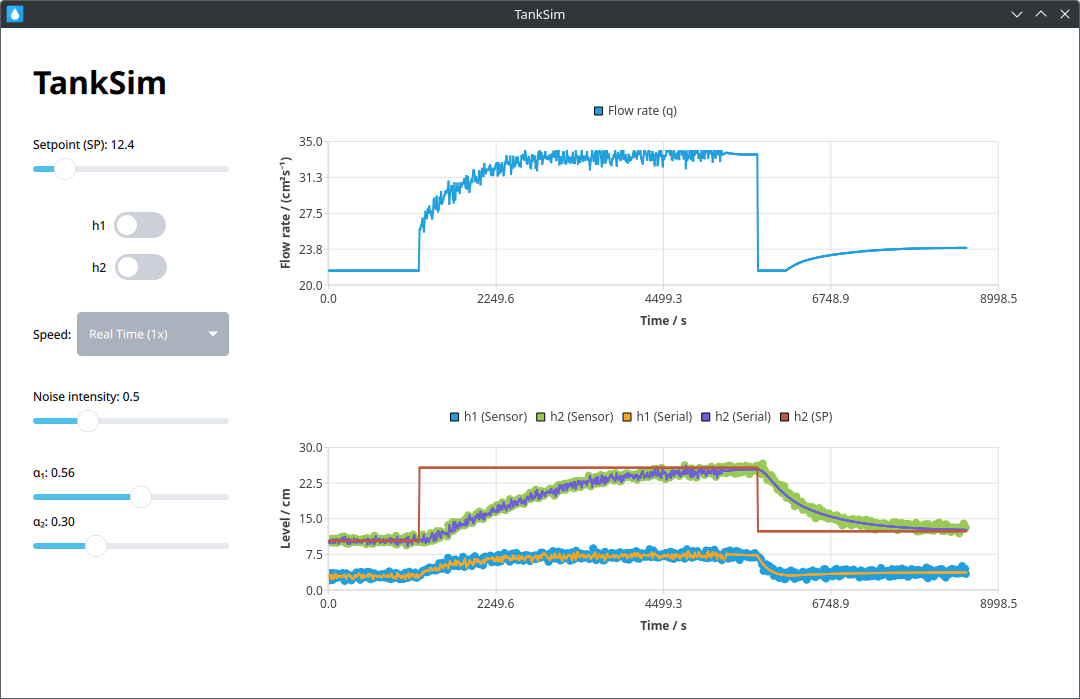
\includegraphics[width=0.45\textwidth]{tanksim.png}
  \caption{Captura de tela do TankSim.}
  \label{fig:interface}
\end{figure}

Este sistema configura-se como um esquema \textit{hardware-in-the-loop} (HIL) \citep{bacic_2005}, no qual o TankSim simula uma planta virtual e envia as leituras dos sensores para o Arduino. Com base nessas informações, o controlador PI implementado no Arduino calcula a ação de controle, ou seja, o novo valor da vazão $q_{\mathrm{in}}$, visando ajustar o nível do tanque $h_2$ até o \textit{setpoint} definido pelo usuário. Em seguida, o Arduino utiliza a PIRNN para prever os valores dos níveis de líquido em cada tanque para o próximo intervalo de tempo. Por fim, o TankSim aplica a ação de controle na planta simulada e exibe os resultados na interface.

Quando os dados dos sensores não estão disponíveis, simulando uma falha ou interrupção manual por meio dos interruptores da interface, o Arduino entra em um modo de retroalimentação. Nesse modo, em vez de receber a entrada do nível anterior dos tanques do simulador, a PIRNN passa a utilizar os valores previstos pela própria rede neural como entrada. Esse mecanismo permite que o sistema continue operando mesmo na ausência de dados dos sensores, garantindo a continuidade da previsão e do controle.

\section{Resultados e Discussão}

A PIRNN apresentou previsões altamente consistentes com a simulação de referência realizada pelo \textit{CasADi} com o método RK4. A Figura \ref{fig:pirnn-results} ilustra os resultados da validação, evidenciando que a PIRNN conseguiu reproduzir com elevada fidelidade a dinâmica do sistema mesmo ao aplicar intensas perturbações na vazão de entrada durante aproximadamente 33 horas de operação.

\begin{figure}[ht]
  \centering
  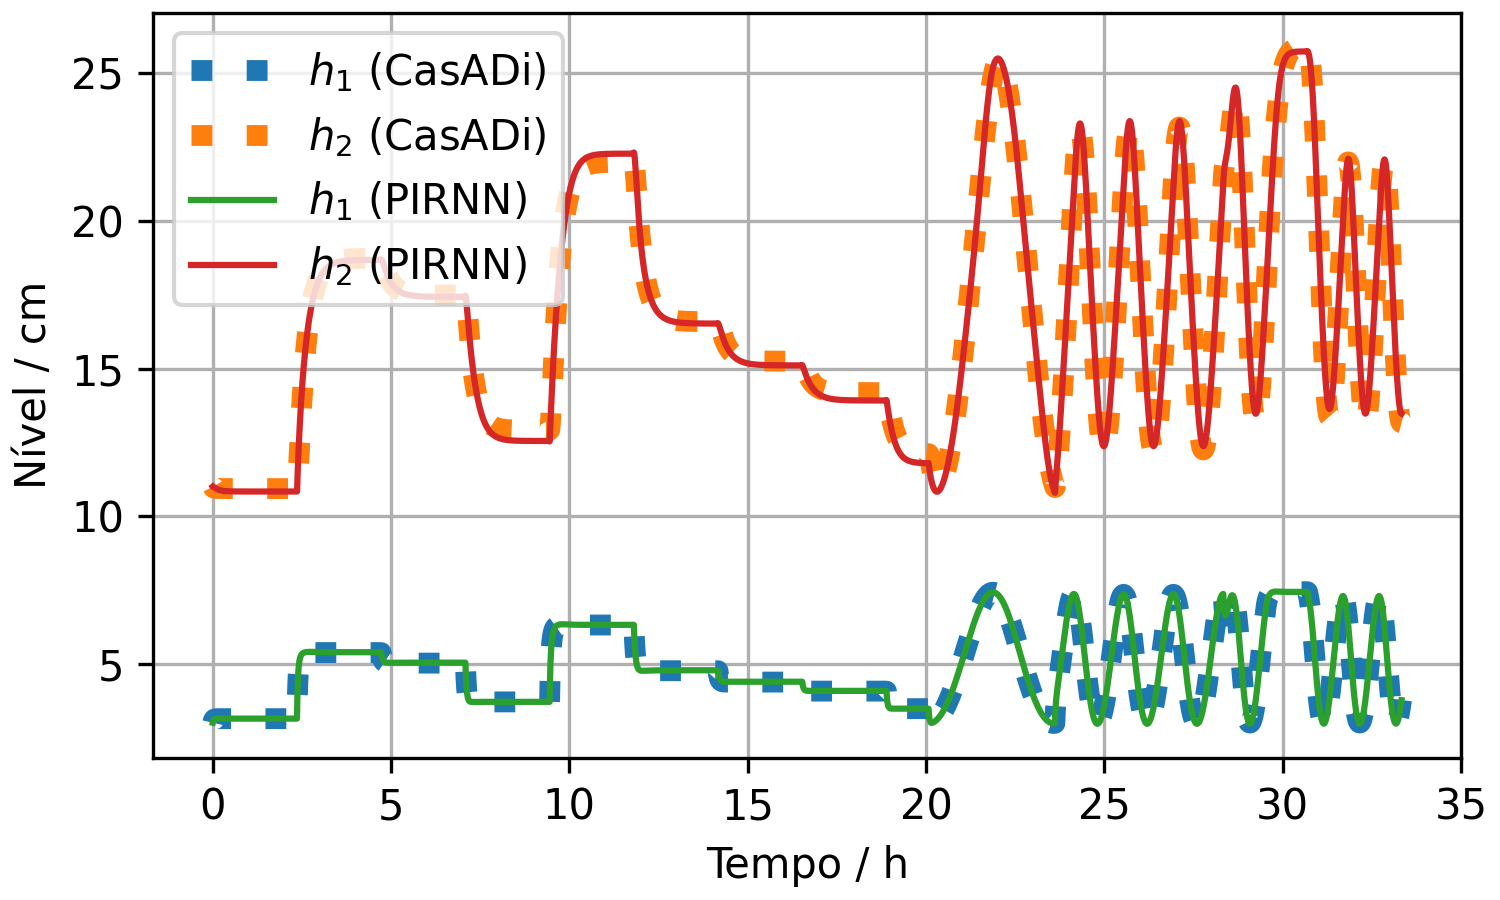
\includegraphics[width=0.45\textwidth]{pirnn-test.png}
  \caption{Comparação entre as previsões da PIRNN e o modelo de referência simulado no \textit{CasADi}.}
  \label{fig:pirnn-results}
\end{figure}

A implementação da PIRNN no Arduino demonstrou um uso eficiente dos recursos computacionais: verificou-se que o programa completo, que inclui a PIRNN, o controlador PI e o código responsável pela comunicação serial com o computador, utilizou 69,1\% da memória flash e apenas 15,9\% da memória RAM do Arduino. Esses números indicam que existem recursos disponíveis para implementação de modelos mais complexos ou execução de tarefas adicionais, caso necessário.

\begin{figure}[ht]
  \centering
  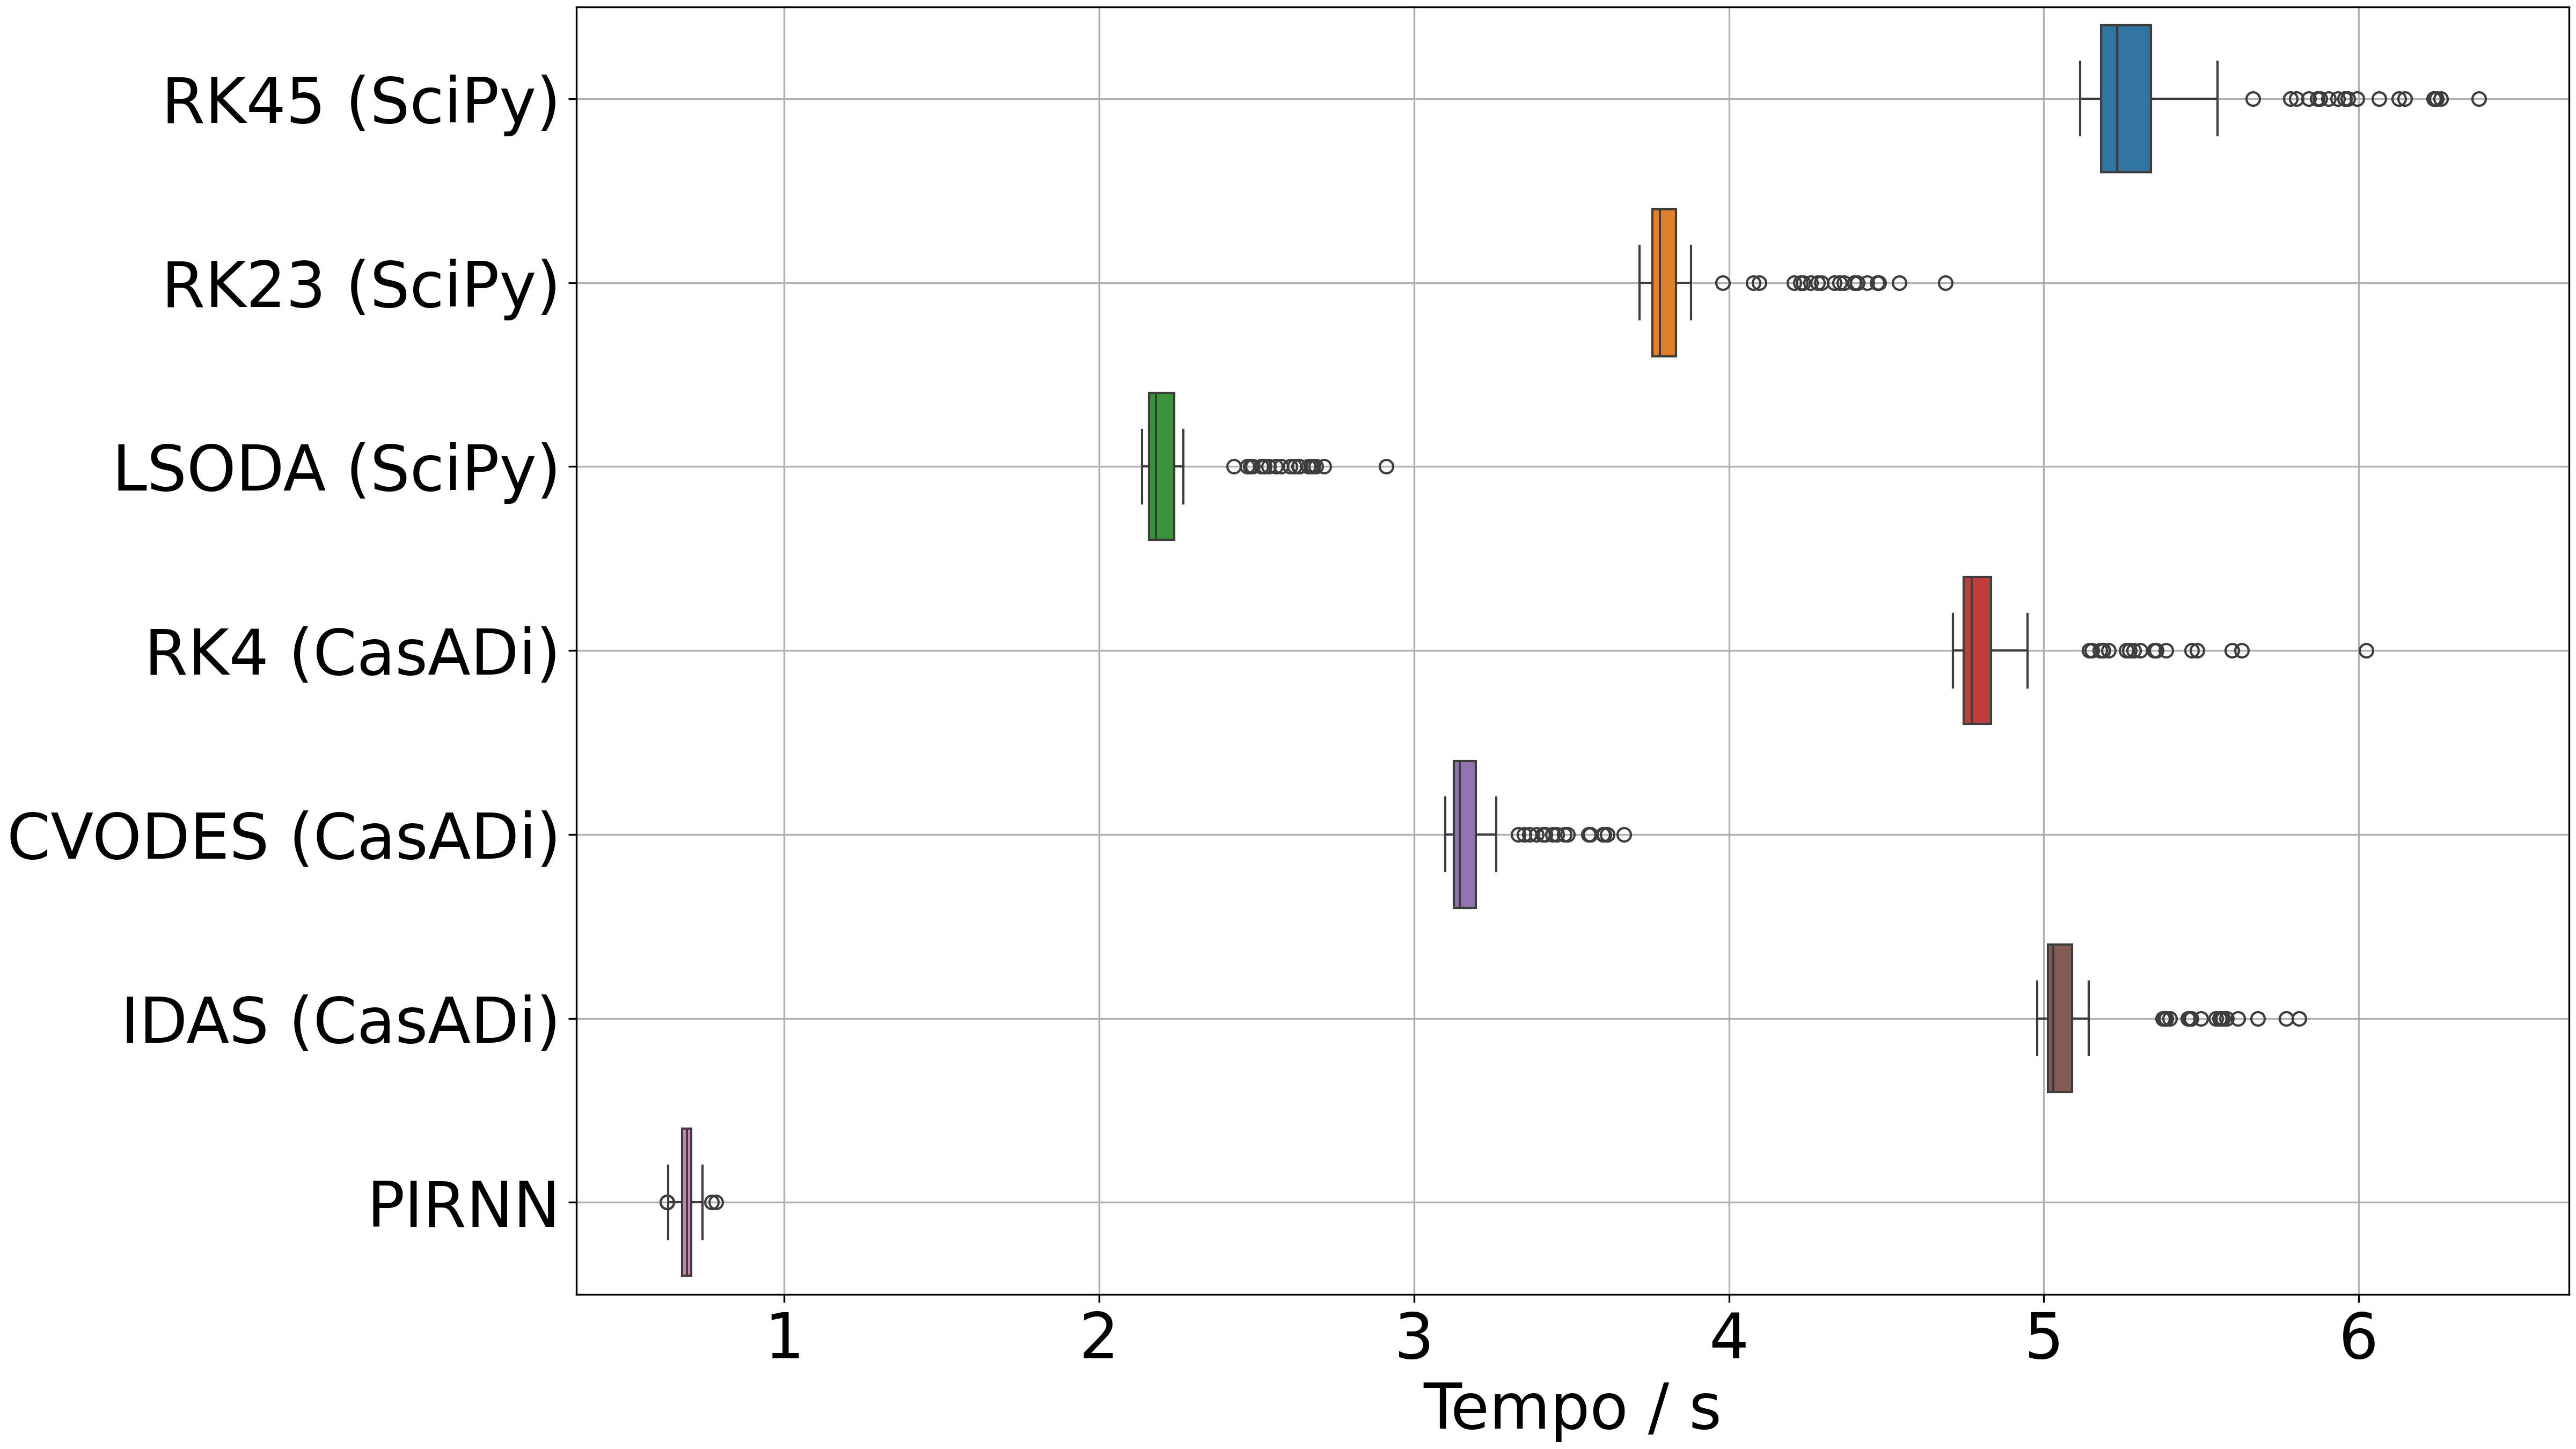
\includegraphics[width=0.45\textwidth]{pirnn-boxplot.png}
  \caption{Boxplot dos tempos de execução dos métodos avaliados.}
  \label{fig:pirnn-benchmark-lite}
\end{figure}

\begin{figure*}[ht]
  \centering
  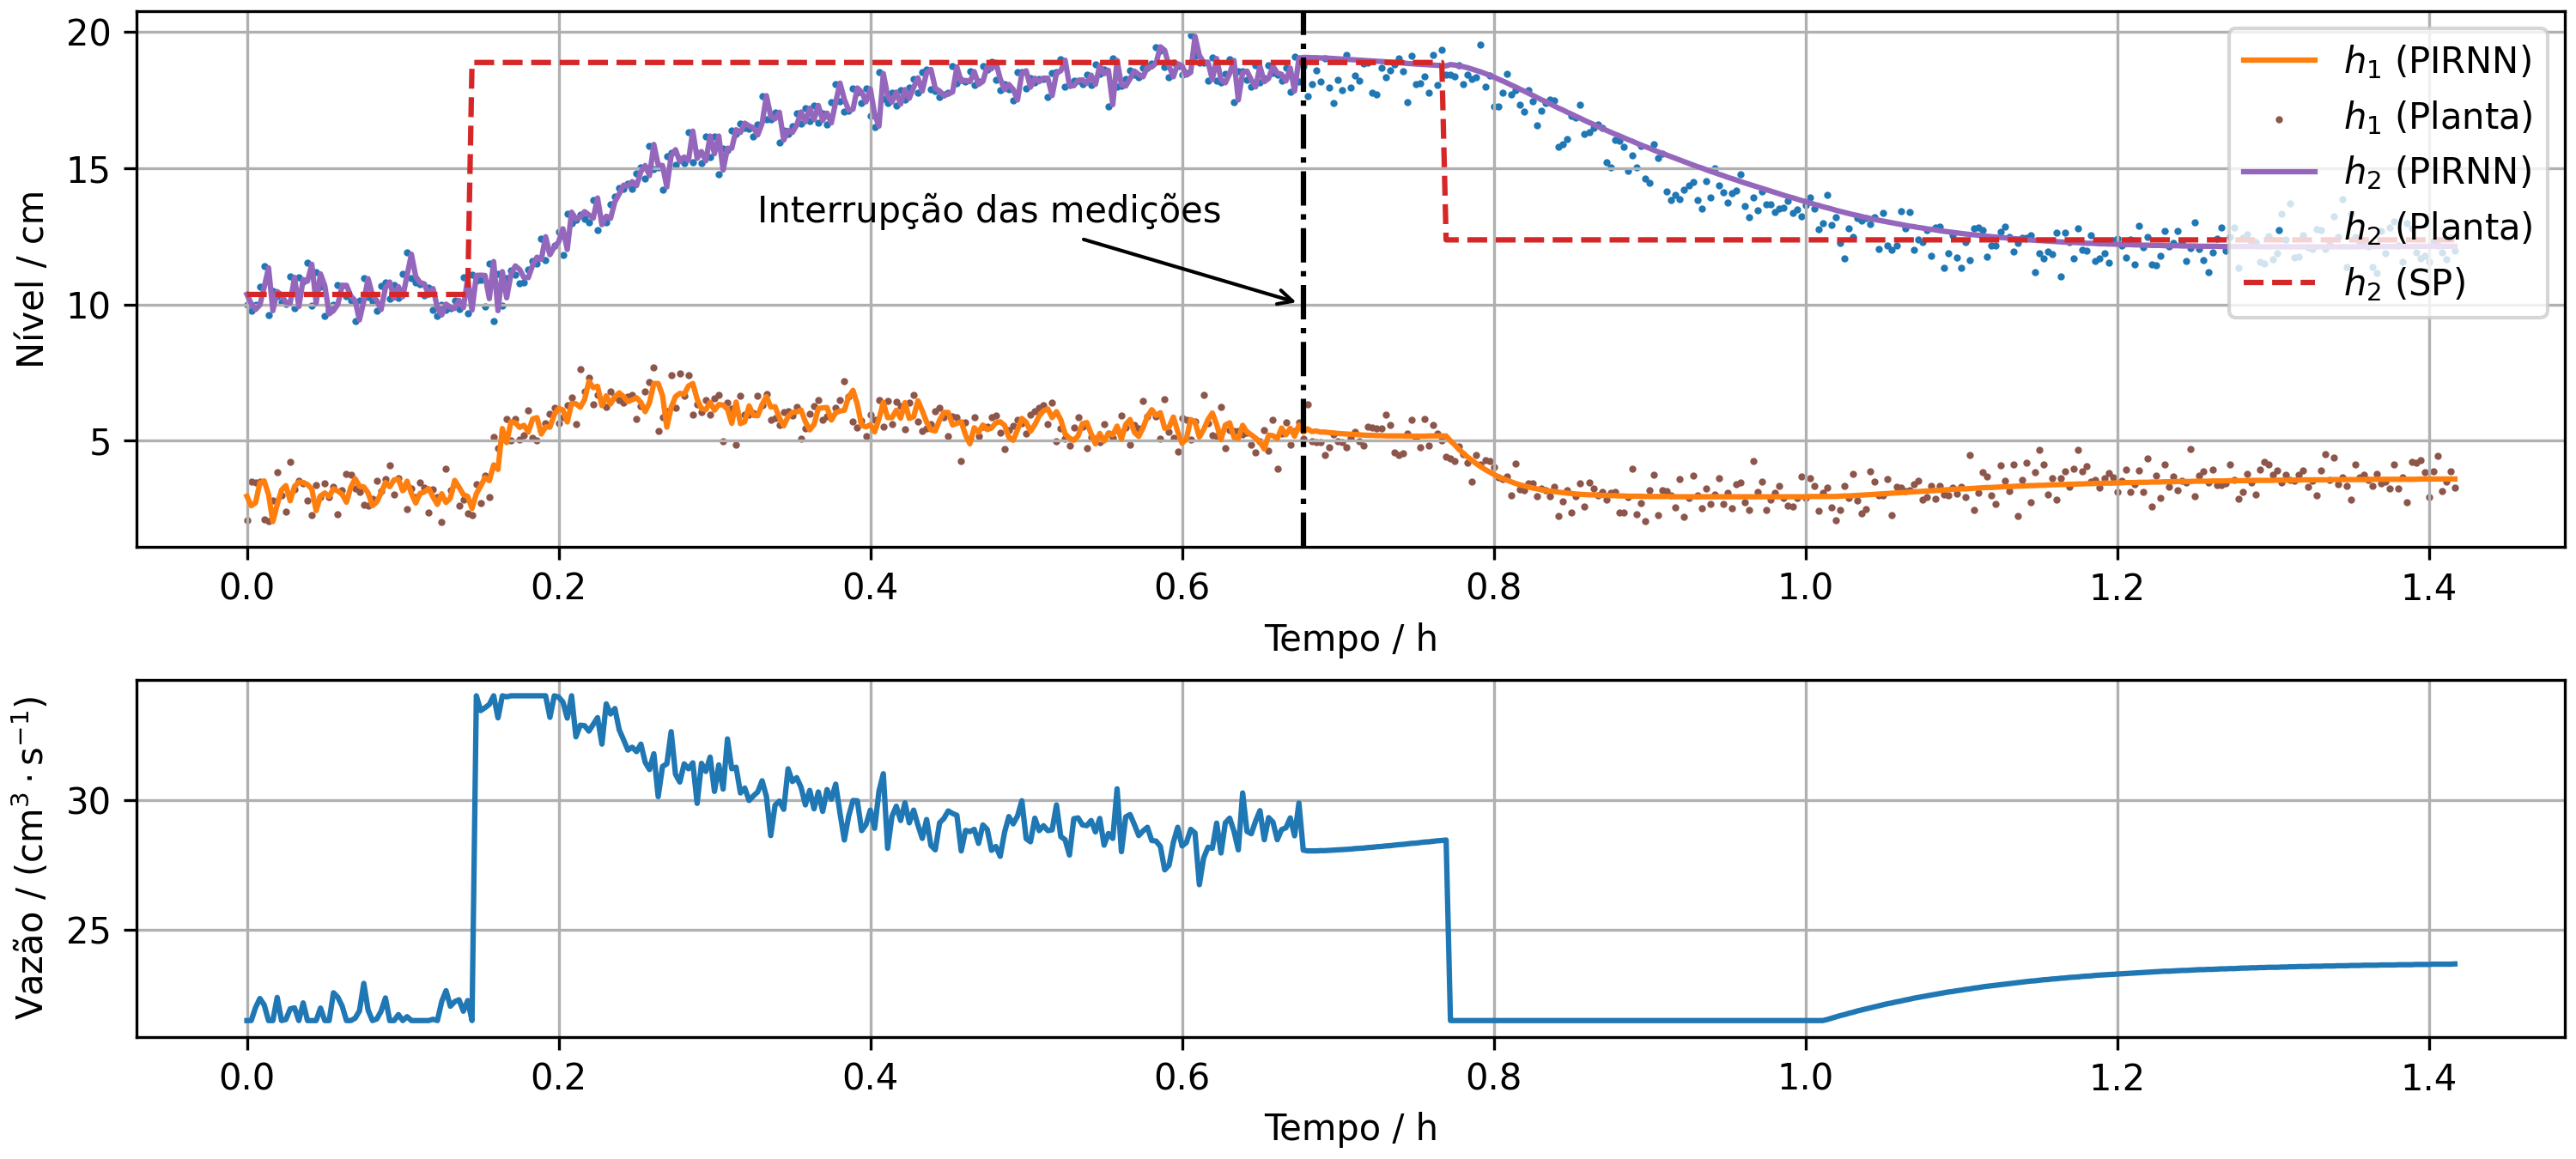
\includegraphics[width=0.8\textwidth]{hil-pirnn-pi.png}
  \caption{Comparação entre as leituras dos sensores, obtidas a partir dos níveis simulados com adição de ruído, e os níveis previstos pela PIRNN embarcada após uma perturbação do tipo degrau na vazão de entrada. A linha preta ponto-traço vertical indica o instante em que os valores dos sensores deixam de ser enviados ao Arduino, fazendo com que a PIRNN passe a se retroalimentar.}
  \label{fig:sil-pirnn}
\end{figure*}

Nos testes de desempenho, a PIRNN demonstrou uma significativa vantagem em termos de velocidade quando comparada com métodos numéricos tradicionais. A comparação foi feita com a implementação dos métodos RK4, CVODES e IDAS da biblioteca \textit{CasADi}, e dos métodos Runge-Kutta de quinta ordem com estimativa de erro de quarta ordem (RK45), Runge-Kutta de terceira ordem com estimativa de erro de segunda ordem (RK23) e LSODA da biblioteca \textit{SciPy}, todos executados no mesmo computador. Para avaliar o desempenho de cada método, foram realizadas 100 execuções de cada algoritmo sob as mesmas condições de entrada utilizadas na validação. A Figura \ref{fig:pirnn-benchmark-lite} apresenta o boxplot dos tempos de cômputo dos métodos avaliados, evidenciando a superioridade da PIRNN em termos de tempo de processamento.

% Local original da imagem pirnn-benchmark-lite

Nos testes de robustez, foram simulados cenários com ruído nas medições e com ausência completa de medições. A Figura \ref{fig:sil-pirnn} apresenta os resultados obtidos nesses testes. Observa-se que no caso de medições ruidosas, a PIRNN capta as variações geradas pelo ruído, mas com um leve amortecimento, sugerindo uma capacidade de filtragem parcial das perturbações. Quando as medições são interrompidas completamente, a PIRNN passa a se retroalimentar. Nesse cenário, ela continua seguindo com precisão o comportamento esperado dos tanques, mesmo sem a entrada de dados dos sensores. Vale destacar que, mesmo nessas condições adversas, o controlador PI implementado no Arduino continua atuando corretamente no sistema, alcançando o \textit{setpoint} com base apenas nas informações fornecidas pela PIRNN.

% Local original da imagem fig:sil-pirnn
\section{Considerações finais}

Neste trabalho, foi demonstrada a utilização de uma PIRNN embarcada em um Arduino UNO atuando como um analisador virtual para medição de nível de um conjunto de tanques.

Os resultados obtidos demonstram que a PIRNN é uma alternativa viável aos métodos numéricos tradicionais, apresentando desempenho superior no tempo de simulação, sem grandes prejuízos à fidelidade das previsões. Outro aspecto relevante é sua robustez, que se mantém mesmo na presença de falhas ou ruídos nas medições. Além disso, sua compatibilidade com plataformas de baixo custo, como o Arduino, torna-a uma solução acessível e eficiente para controle em tempo real, com aplicações potenciais em automação industrial, monitoramento de processos e como analisador virtual.

Contudo, em sistemas dinâmicos reais, é necessário considerar a degradação dos parâmetros do modelo ao longo do tempo, causada pelo desgaste ou envelhecimento dos componentes físicos. Essa degradação pode comprometer o desempenho da PIRNN, tornando necessário o retreinamento periódico do modelo para garantir sua acurácia. Nesse contexto, estudos futuros podem explorar técnicas de aprendizado por reforço, visando a adaptação em tempo real da PIRNN às mudanças dos parâmetros do sistema sem a necessidade de intervenções manuais.

Por fim, pesquisas adicionais podem investigar a implementação de modelos mais complexos, visando expandir a aplicabilidade das PIRNNs em sistemas dinâmicos descritos por equações diferenciais parciais.


\section*{Agradecimentos}
Os autores gostariam de agradecer o suporte financeiro da ANP no âmbito do PRH 35.1.

\bibliography{../common/bibliography.bib}

\end{document}
